\newif\ifuseseminar
\useseminarfalse
\input{../../latex_common/header.tex.frag}

\title{Análise vetorial de Gibbs}

\begin{document}
\section{Espaço vetorial}

\subsection{Definições}

Os espaços vetoriais são usados na física para representar as mais diversas
quantidades. Por exemplo, na mecânica Newtoniana usamos espaços vetoriais para
representar posições no espaço, velocidades e deslocamentos. Vale ressaltar que
essas três quantidades físicas tem naturezas distintas e isso se reflete no
significado das operações que podemos fazer com elas. Por exemplo, vetores
velocidade podem ser somados ou subtraídos quando queremos representar
velocidades em diferentes referenciais inerciais. De maneira similar, vetores
posição podem ser somados quando fazemos uma mudança da origem de um sistema de
coordenadas. Contudo, não há significado natural para a soma de um vetor posição
e um vetor velocidade, mesmo que essa soma seja bem definida
matematicamente.\footnote{Naturalmente, nesse caso teríamos um problema de
	unidades, o que é mais um sinal de que estamos tratando de espaços diferentes.}
Isso evidencia que quando trabalhamos com análise vetorial, estamos geralmente
tratando de vários espaços vetoriais diferentes. Isso se torna mais evidente
quando trabalhamos com coordenadas curvilíneas, como veremos mais adiante.

Para tornarmos nossa discussão mais rigorosa, começamos por definir espaços
vetoriais. No nosso tratamento vamos nos restringir à espaços vetoriais reais,
isto é, nossos espaços vetoriais se darão sobre o corpo dos reais $\mathbb{R}$.
Na prática, isso significa que podemos multiplicar nosso vetores por números
reais. Porém, antes de definirmos espaços vetoriais, vamos introduzir alguns
conceitos matemáticos mais básicos que serão úteis ao longo de toda exposição.
Esses conceitos podem parecer demasiadamente formais e desnecessários para a
compreensão do assunto, porém é importante que o estudante tenha à sua
disposição essas definições para que em qualquer momento ele possa consultá-las
e esclarecer o significado das demais expressões usadas nessa exposição.

\definition{Produto
	cartesiano, dado dois conjuntos $A$ e $B$, o produto cartesiano é simplesmente o
	conjunto dos pares ordenados da forma
	$$A\times B \equiv \set{(a,b),a\in A \;\mathrm{and}\; b\in B}.$$}

\definition{Função entre conjuntos, sejam $A$ e $B$ dois conjuntos, denotamos
	por $$f:A \to B.$$ a função $f$ com domínio $A$ e imagem $B$. Usamos a
	notação $f(a) \in B $ para designar o valor da função $f$ quando aplicada ao
	elemento $a \in A$. É importante ressaltar que algumas funções são denotadas de
	forma diferente, por exemplo, a função soma de reais
	$+:\mathrm{R}\times\mathrm{R}\to \mathrm{R}$ é representada como $a+b \in
		\mathrm{R}$ para $a,b\in\mathrm{R}$. Nesses casos costumamos chamar essas
	funções de operadores.\label{def:func}}

Na Def.~\ref{def:func} vimos que utilizamos uma notação diferente para denotar
algumas funções, como no exemplo a soma de dois números reais. Além disso,
alguma funções são ainda mais simplificadas, por exemplo, a multiplicação de
dois números reais é normalmente designada pela mera justaposição de dois
números. Ou seja, quando escrevemos $ab$ onde $a,b\in \mathrm{R}$ estamos
escrevendo de forma compacta a aplicação da função multiplicação à dois números
reais.

Finalmente, podemos definir o conceito de espaço vetorial real:
\definition{Um espaço vetorial sobre os reais $\mathbb{R}$ é dado por um
	conjunto $\mathbb{V}$ e dois produtos, multiplicação por escalar e a soma de
	dois vetores. Os elementos de $\mathbb{V}$ serão descritos por um seta acima do
	símbolo, ou seja, $\vec{v} \in \mathbb{V}$. Os produtos são dados por:
	$$\cdot:\mathbb{R}\times\mathbb{V} \to  \mathbb{V}\quad\quad +:\mathbb{V}\times\mathbb{V}\to \mathbb{V}. $$
	O produto soma $+$ possui as seguintes propriedades (onde $\vec{v},\vec{u},\vec{w}\in \mathbb{V}$):
	\begin{enumerate}
		\item Associatividade: $\left(\vec{v}+\vec{u}\right)+\vec{w} = \vec{v}+\left(\vec{u}+\vec{w}\right)$.
		\item Comutatividade: $\vec{v}+\vec{u} = \vec{u}+\vec{v}$.
		\item Existência do elemento neutro (identidade aditiva): $\vec{v}+\vec{0} = \vec{v}$.
		\item Existência do inverso aditivo: $\vec{v}+(-\vec{v}) = \vec{0}, \quad -\vec{v} \in \mathrm{V}$.
	\end{enumerate}
	O produto multiplicação por reais satisfaz (note que iremos denotar esse
	produto pela simples justaposição de um real e um vetor, temos também que $\vec{v},\vec{u} \in \mathbb{V}$ e $a,b\in\mathbb{R}$):
	\begin{enumerate}
		\item Compatibilidade da multiplicação entre reais e reais e vetores: $a(b\vec{v}) = (ab)\vec{v}$.
		\item Existência do elemento neutro (identidade multiplicativa): $1\vec{v} = \vec{v}$.
		\item Distributividade sob multiplicação por reais: $a(\vec{v}+\vec{u}) = a\vec{v}+a\vec{u}$.
		\item Distributividade sob adição de reais: $(a+b)\vec{v} = a\vec{v}+b\vec{v}$.
	\end{enumerate}
	\label{vecspace}
}

Um primeiro exemplo óbvio de espaços vetoriais reais é o próprio conjunto dos
reais $\mathbb{R}$, chamamos os elementos desse espaço de escalares. É fácil
checar que esse conjunto satisfaz todas as propriedades descritas acima. Podemos
usar esse fato para construirmos espaços vetoriais mais complicados. Considere o
produto cartesiano de dois espaços reais, $\mathbb{R}^2 \equiv
	\mathbb{R}\times\mathbb{R}$. Agora, podemos $\mathbf{definir}$ a soma de dois
elementos de $\mathbb{R}$ e a multiplicação por um número real como,
\begin{align}
	(a,b) + (c,d) & \equiv (a + c, b+d), \quad a,b,c,d \in \mathbb{R}, \\
	a(b,c)        & \equiv (ab, ac), \quad a,b,c\in\mathbb{R}.
\end{align}
Novamente, é fácil checar que todas propriedades da Def.~\ref{vecspace} são
automaticamente respeitadas. É interessante perceber exatamente o que estamos
fazendo, ao definir a soma e a multiplicação como acima, estamos usando os
conceitos de soma e multiplicação de números reais e estamos usando eles para
definir soma e multiplicação em conjuntos mais complicados, no caso
$\mathbb{R}^2$. Em outras palavras, o conjunto dos pares ordenados de números
reais forma um espaço vetorial uma vez que definimos as operações acima.
Naturalmente, podemos fazer as mesmas definições para $\mathbb{R}^3 \equiv
	\mathbb{R}\times\mathbb{R}\times\mathbb{R}$. Daqui para a frente, vamos sempre
usar essas definições de soma e multiplicação por escalar quando tratarmos de
espaços $\mathbb{R}^n \equiv
	\mathbb{R}\times\mathbb{R}\times\dots\times\mathbb{R}$.

\subsection{Independência linear}

Para demarcar a diferença entre $\mathbb{R}^2$ e $\mathbb{R}^3$, apresentamos
uma nova definição:
\definition{Independência linear: um conjunto de vetores
	$\vec{v}_i,\;i\in(1,2,\dots, n)$ é dito linearmente independentes se a sua
	combinação linear for nula se e somente se todos os coeficiente forem nulos,
	i.e.,
	$$\sum_{i=1}^n a^i\vec{v}_i = 0,\;\text{se e somente se}\; a^i=0\;\forall\; i\in(1,2\dots,n).$$
}

Em termos práticos um conjunto de vetores é linearmente independente se um dos
vetores não pode ser escrito como combinação dos outros, ou seja, quando eles
\textbf{não} são linearmente independentes, a combinação pode ser zero mas os
coeficientes podem não ser todos zero (digamos que $a^1 \neq 0$) então
\begin{equation}
	\vec{v}_1 = -\frac{1}{a^1}\sum_{i=2}^n a^i\vec{v}_i.
\end{equation}
\definition{Dizemos que um conjunto de vetores forma uma base eles forem
	linearmente independentes e se qualquer elemento de $\mathbb{V}$ pode ser
	escrito como uma combinação linear deles. O número de vetores na base denota a
	dimensão de $\mathbb{V}$.}

É fácil checar que os vetores $\vec{e}_1 \equiv (1,0,0)$, $\vec{e}_2 \equiv
	(0,1,0)$ e $\vec{e}_3 \equiv (0,0,1)$, formam uma base em $\mathbb{R}^3$. Por
isso, qualquer vetor nesse espaço pode ser escrito como uma combinação desses
vetores, i.e.,
\begin{equation}
	\vec{v} = \sum_{i=1}^n v^i\vec{e}_i.
\end{equation}
Do ponto de vista da física, estamos interessados em usar conceitos matemáticos
para representar elementos concretos encontrados na natureza. Nossa experiência
no mundo real nos mostra que precisamos de três coordenadas para marcar um ponto
no espaço. Se calcularmos as três coordenadas de um objeto em relação a uma
origem e depois as coordenadas da posição da origem em relação a outro ponto de
referência, temos que a posição do objeto em relação ao outro ponto de
referência é dada pela simples soma das coordenadas.  Esse exemplo mostra que
podemos mapear o conceito de posição no espaço nos elementos de $\mathbb{R}^3$,
mas não só isso, que as operações definidas nesse espaço têm também sentido
físico. Nesse sentido, é importante entender o que fazemos quando aplicamos uma
modelagem física: estamos procurando objetos matemáticos que possam ser mapeados
em quantidades físicas e que suas operações correspondam à elementos do mundo
físico. No exemplo acima, os pontos de $\mathbb{R}^3$ são mapeados em pontos
coordenadas de posições no mundo real e a soma de dois vetores à mudança da
origem das coordenadas.

Neste capítulo vamos nos ater a espaços vetoriais de três dimensões, que é a
arena onde o eletromagnetismo será desenvolvido nesse curso.

\begin{Exercise}[label=dim, title={Espaço vetorial}]
	\vspace{-\baselineskip}%
	\Question Mostre que $\mathbb{R}^2$ e $\mathbb{R}^3$, são espaços
	vetoriais de dimensão dois e três respectivamente.
\end{Exercise}

\section{Produto interno}
\subsection{Definição e propriedades}

O produto interno é definido como uma função atuando em um espaço vetorial que
serve para calcular tamanhos e ângulos entre vetores. Em geral a definição
matemática é:
\definition{Produto interno: dado um espaço vetorial $\mathbb{V}$ definimos o
	produto interno como o mapa
	$$\cdot:\mathbb{V}\times\mathbb{V}\to \mathbb{R}.$$
	Que satisfaz as seguintes propriedades (onde $\vec{v},\,\vec{u},\,\vec{w}\in\mathbb{V}$):
	\begin{enumerate}
		\item Simetria: $\vec{v}\cdot\vec{w} = \vec{w}\cdot\vec{v}$.
		\item Linearidade a esquerda: $(\vec{v}+\vec{u})\cdot\vec{w} = \vec{v}\cdot\vec{w}+\vec{u}\cdot\vec{w}$.
		\item Positividade: $\vec{v}\cdot\vec{v} \geq 0$ e só é igual a zero se e somente se $\vec{v}=\vec{0}$.
	\end{enumerate}
	Vale ressaltar que a linearidade a esquerda em conjunto com a simetria, implica
	linearidade a direita. Em outras palavras, esse produto é bilinear. Finalmente,
	dado um produto interno, definimos a norma ou comprimento de um vector como
	\begin{equation}
		\vert\vec{v}\vert \equiv \sqrt{\vec{v}\cdot\vec{v}},
	\end{equation}
	onde a positividade garante que a raiz quadrada é sempre bem definida.
}

Em geral, existem inúmeras escolhas diferentes para produtos internos. Para ver
isso, podemos notar que a linearidade implica que o produto de quaisquer dois
vetores é
$$ \vec{v}\cdot\vec{u} = \left(\sum_{i=1}^3v^i\vec{e}_i\right)\cdot \left(\sum_{j=1}^3u^j\vec{e}_j\right) = \sum_{i,j=1}^3v^iu^j \;\vec{e}_i\cdot\vec{e}_j.$$
Isto é, podemos calcular o produto interno entre quaisquer dois vetores se
conhecermos o produto interno entre os elementos da base. Para determinar esse
produto, precisamos então definir as seis quantidades $\vec{e}_i\cdot\vec{e}_j$,
note que em geral teríamos nove combinações de $i$ e $j$ mas a simetria nos dá
três equações
\begin{equation}
	\vec{e}_2\cdot\vec{e}_1 = \vec{e}_1\cdot\vec{e}_2, \qquad \vec{e}_3\cdot\vec{e}_1 = \vec{e}_1\cdot\vec{e}_3, \qquad \vec{e}_3\cdot\vec{e}_2 = \vec{e}_2\cdot\vec{e}_3.
\end{equation}
A menos da imposição da positividade,\footnote{Essa condição impõe limitações
	sobre os sinais e relações de desigualdades entre os termos, porém, não impõe
	nenhuma equação adicional e, portanto, não reduz a dimensão do problema.} temos
total liberdade para escolher essas seis quantidades.

\subsection{Delta de Kronecker}

No nosso tratamento, supomos que o espaço é plano e, nesse caso, o produto interno
que reproduz a geometria Euclidiana que conhecemos é dado por
$\vec{e}_i\cdot\vec{e}_j = \delta_{ij}$. Onde introduzimos o delta de Kronecker,
\begin{equation}
	\delta_{ij} \equiv \left\{ \begin{array}{cc}
		1 & \text{se}\; i=j     \\
		0 & \text{se}\; i\neq j\end{array} \right..
\end{equation}
Nessas notas o produto interno será sempre dado pelo produto Euclideano definido
acima.

Para entendermos o significado geométrico desse produto começamos por calcular o
comprimento de um vetor,
\begin{equation}
	\vert\vec{v}\vert = \sqrt{(v^1)^2+(v^2)^2+(v^3)^2},
\end{equation}
que é simplesmente a norma Euclidiana que já conhecemos. Podemos agora definir
(implicitamente) o angulo $\theta$ entre dois vetores da forma
\begin{equation}
	\vec{v}\cdot\vec{u} = \vert\vec{v}\vert\vert\vec{u}\vert \cos\theta.
\end{equation}
Para vermos que essa definição coincide com as definições usuais da geometria
Euclidiana, tome o produto entre o vetor $\vec{v} = a^1\vec{e}_1+a^2\vec{e}_2$
com o vetor $\vec{u} = \vec{e}_1$, i.e.,
\begin{equation}
	\vec{v}\cdot\vec{u} = \left(a^1\vec{e}_1+a^2\vec{e}_2\right)\cdot \vec{e}_1 = a^1 = \vert\vec{v}\vert\vert\vec{u}\vert \frac{a^1}{\sqrt{(a^1)^2+(a^2)^2}} \Rightarrow \cos\theta = \frac{a^1}{\sqrt{(a^1)^2+(a^2)^2}}.
\end{equation}
Ou seja, no exemplo acima o cosseno do ângulo entre os vetores é exatamente o
cateto adjacente sobre a hipotenusa.

Em geral o produto interno definido anteriormente pode ser escrito como
\begin{equation}\label{prodint}
	\vec{v}\cdot\vec{u} = \left(\sum_{i=1}^3v^i\vec{e}_i\right)\cdot \left(\sum_{j=1}^3u^j\vec{e}_j\right) = \sum_{i,j=1}^3v^iu^j \;\vec{e}_i\cdot\vec{e}_j = \sum_{i,j=1}^3v^iu^j \; \delta_{ij} = \sum_{i=1}^3v^iu^i.
\end{equation}
Vale ressaltar que na última igualdade acima usamos o fato de que $\delta_{ij} =
	0$ para $i \neq j$ para eliminar um somatório. Por fim, dizemos que dois vetores
$\vec{v}$ e $\vec{u}$ são ortogonais se $\vec{v}\cdot\vec{u} = 0$.

Usando a norma de um vetor, definimos o vetor unitário associado a $\vec{v}$ da
seguinte forma,
\begin{equation}
	\hat{v} \equiv \frac{\vec{v}}{\vert\vec{v}\vert}.
\end{equation}

\begin{Exercise}[title={Produto interno}]
	\vspace{-\baselineskip}%
	\Question Mostre que linearidade a esquerda e simetria implicam linearidade
	a direita.
	\Question Escreva explicitamente os somatórios acima e mostre que a
	presença do delta de Kronecker pode ser usado para eliminar um somatório.
\end{Exercise}

\section{Produto vetorial}
\subsection{Produto externo}
\label{sec:eprod}

A analise vetorial que desenvolvemos até aqui diz respeito a objetos que
representam pontos e direções no espaço. Porém, existem outros conceitos que
podem ser necessários para descrever um fenômeno físico, a saber planos e
volumes. Note que para descrever um plano, precisamos de duas direções no
espaço, ou seja, existe somente um plano contido por dois vetores que não sejam
colineares.\footnote{Vetores colineares são aqueles correspondem a uma simples
	multiplicação por escalar, ou seja, se $\vec{v}$ e $\vec{u}$ são colineares
	então, existe um número real $a \neq 0$ tal que $\vec{v}=a\vec{u}$.} Já um
volume precisa de três vetores, que não sejam colineares entre sí, para ser
definido. O conceito necessário para definirmos planos e volumes é o de produto
tensorial. Nessa exposição faremos uma discussão simplificada sobre esse tema
para desenvolver a intuição do leitor. Falando livremente, o produto tensorial
de um espaço $\mathbb{V}$ com ele mesmo ($\mathbb{V}\otimes\mathbb{V}$) é também
um espaço vetorial (no sentido da Def.~\ref{vecspace}) formado pelos vetores de
base $\vec{e}_i\otimes \vec{e}_j,\;i,j\in (1,2,3)$, ou seja, é um espaço
vetorial de dimensão nove (9). Contudo, para descrevermos planos e volumes
queremos excluir o caso com vetores colineares, para tanto, basta nos
restringirmos ao subespaço antissimétrico de ($\mathbb{V}\otimes\mathbb{V}$),
fazemos essa escolha pois o produto antissimétrico de dois vetores colineares é
sempre nulo.
\definition{A base desse espaço tensorial antissimétrico de
	segunda ordem definida como
	\begin{equation}
		\vec{e}_i\wedge \vec{e}_j\in\mathbb{V}\wedge\mathbb{V},\quad \vec{e}_i\wedge \vec{e}_j = \left(\vec{e}_i\otimes \vec{e}_j - \vec{e}_j\otimes \vec{e}_i\right).
	\end{equation}}

Denotamos vetores no espaço $\mathbb{V}\wedge\mathbb{V}$ de bivetores. Nessa
definição usamos o produto externo, nessa apresentação não entraremos nos
detalhes matemáticos necessários para sua definição formal. As propriedades
importantes no nosso contexto são:
\begin{equation}
	\begin{split}
		\vec{v}\wedge\vec{u}                           & = - \vec{u}\wedge\vec{v},\quad (\vec{v}+\vec{u})\wedge\vec{w} = \vec{v}\wedge\vec{w}+\vec{u}\wedge\vec{w}, \quad (a\vec{v})\wedge\vec{u} = a\vec{v}\wedge\vec{u},, \\
		\left(\vec{v}\wedge\vec{u}\right)\wedge\vec{w} & = \vec{v}\wedge\left(\vec{u}\wedge\vec{w}\right),\quad \vec{v},\;\vec{u},\;\vec{w}\in\mathbb{V},\;a\in\mathbb{R}.
	\end{split}
\end{equation}
É fácil checar que esse espaço é de dimensão três, ou seja, só existem três
vetores de base não nulos ($\vec{e}_1\wedge \vec{e}_2$, $\vec{e}_1\wedge
	\vec{e}_3$, $\vec{e}_2\wedge \vec{e}_3$). É por causa dessa coincidência, de que
o número de dimensões do espaço dos tensores anti-simétricos em três dimensões é
também três, que J. Willard Gibbs introduz no seu livro texto de analise
vetorial o conceito de produto vetorial. A ideia é que podemos criar um mapa
linear e biunívoco entre o espaço $\mathbb{V}\wedge\mathbb{V}$ e o espaço
vetorial original $\mathbb{V}$, em outras palavras um isomorfismo entre
$\mathbb{V}\wedge\mathbb{V}$ e $\mathbb{V}$. Para isso, note que só existe um
vetor ortogonal ao plano $\vec{e}_1\wedge\vec{e}_2$ (isto é, um vetor que é
ortogonal a ambos os vetores usados para construir o plano), o vetor
$\vec{e}_3$.

\subsection{Definição}

Para definirmos nosso mapa, podemos então fazer $\vec{e}_1\wedge\vec{e}_2 \to
	\vec{e}_3$, porém, note que os planos podem ter diferente sinais (e.g.,
$\vec{e}_1\wedge\vec{e}_2 = -\vec{e}_2\wedge\vec{e}_1$). Ou seja, para
determinarmos nosso mapa precisamos escolher os sinais dos planos que são
mapeados nos vetores. Aqui, seguiremos a escolha usual da ``regra da mão
direita'',\footnote{Note que essa é uma escolha arbitrária, em princípio
	qualquer outra escolha é possível. Contudo, para evitar confusão existe uma
	convenção universal.} escolhemos o sinal de acordo com a posição do polegar da
mão direita quando alinhamos o primeiro vetor do produto a palma da mão e o
segundo as pontas dos dedos, i.e., definimos o mapa linear
$V:\mathbb{V}\wedge\mathbb{V}\to\mathbb{V}$ da forma
\begin{equation}\label{vecprod}
	V(\vec{e}_1\wedge\vec{e}_2) = \vec{e}_3, \quad V(\vec{e}_3\wedge\vec{e}_1) = \vec{e}_2, \quad V(\vec{e}_2\wedge\vec{e}_3) = \vec{e}_1.
\end{equation}
Vamos agora calcular explicitamente o produto de dois vetores e calcular seu
mapa para o espaço $\mathbb{V}$.,
\begin{equation}\label{wedprod}
	\begin{split}
		\vec{v}\wedge\vec{u} & = \left(\sum_{i=1}^3v^i\vec{e}_i\right)\wedge\left(\sum_{j=1}^3u^j\vec{e}_j\right),                                                                         \\
		                     & = \left(v^1u^2-v^2u^1\right)\vec{e}_1\wedge\vec{e}_2-\left(v^1u^3-v^3u^1\right)\vec{e}_3\wedge\vec{e}_1+\left(v^2u^3-v^3u^2\right)\vec{e}_2\wedge\vec{e}_3.
	\end{split}
\end{equation}
Finalmente, definimos o produto vetorial aplicando o nosso isomorfismo $V$ a
esse produto,
\begin{equation}\label{vprod}
	\vec{v}\times\vec{u} \equiv V(\vec{v}\wedge\vec{u}) =\left(v^2u^3-v^3u^2\right)\vec{e}_1-\left(v^1u^3-v^3u^1\right)\vec{e}_2+ \left(v^1u^2-v^2u^1\right)\vec{e}_3.
\end{equation}
Para simplificar os cálculos de produtos vetoriais, podemos calcular o produto
dos vetores de base e estabelecer uma regra geral, para tanto escrevemos
\begin{equation}\label{levicivita}
	\vec{e}_i\times\vec{e}_j = \sum_{k=1}^3\epsilon_{ijk}\vec{e}_k.
\end{equation}
A antissimetria do produto vetorial mostra que o termo $\epsilon_{ijk}$, que
chamamos de símbolo de Levi-Civita, deve ser antissimétrico nas suas duas
primeira componentes  $\epsilon_{ijk} = -\epsilon_{jik}$. Ademais, examinando a
Eq.~\eqref{vecprod} vemos que esse símbolo também é antissimétrico nos dois
últimos índices, i.e., $\epsilon_{ijk} = -\epsilon_{ikj}$ e que $\epsilon_{123}
	= 1$. Usando o símbolo de Levi-Civita podemos escrever a Eq.~\eqref{vprod} de
forma mais compacta,
\begin{equation}\label{vpe}
	\vec{v}\times\vec{u} = \left(\sum_{i=1}^3v^i\vec{e}_i\right)\times\left(\sum_{j=1}^3u^j\vec{e}_j\right)=\sum_{ijk}^3\epsilon_{ijk}v^iu^j\vec{e}_k.
\end{equation}
Não só a forma acima é mais compacta mas ela é muito mais conveniente para
calcularmos produtos mais complicados como veremos mais a diante.

Do ponto de vista geométrico, podemos entender o significado desse produto,
calculando o produto vetorial entre o vetor $\vec{v} =\vec{e}_1
$ com o vetor $\vec{u} = a^1\vec{e}_1+a^2\vec{e}_2$,
\begin{equation}
	\vec{v}\times\vec{u} = a^2\vec{e}_3 = \vert\vec{v}\vert\vert\vec{u}\vert \frac{a^2}{\sqrt{(a^1)^2+(a^2)^2}}\vec{e}_3 = \vert\vec{v}\vert\vert\vec{u}\vert \sin\theta\;\vec{e}_3.
\end{equation}
Em outras palavras, o produto vetorial de dois vetores resulta em um vetor
ortogonal ao plano formado e com norma igual a área do paralelogramo formado
pelos dois vetores. Veja que isso deixa evidente que o resultado de um produto
vetorial não tem o mesmo significado físico de um vetor ordinário, na nossa
construção deixamos claro que o produto vetorial é na verdade um produto
tensorial antissimétrico, usado para representar planos (logo o sua norma está
associada a áreas e não a comprimentos), mas que em três dimensões tem a mesma
dimensionalidade do espaço vetorial original e por isso fazemos um mapa entre
esses espaços.

O caso dos volumes é ainda mais simples, seguindo a lógica anterior, queremos a
composição de três vetores que não sejam colineares, nesse caso queremos o
produto tensorial antissimétrico $\mathbb{V}\wedge\mathbb{V}\wedge\mathbb{V}$,
que chamamos de espaço dos trivetores. O único vetor de base nesse espaço é
$\vec{e}_1\wedge\vec{e}_2\wedge\vec{e}_3$, qualquer outra combinação é nula ou
proporcional a esse vetor devido a antissimetria do produto. Isso mostra que
esse espaço é unidimensional. Por essa razão podemos mapear esse espaço no
próprio $\mathbb{R}$ usando o mapa $\Upsilon:
	\mathbb{V}\wedge\mathbb{V}\wedge\mathbb{V}\to\mathbb{R}$, definido por
$\Upsilon(\vec{e}_1\wedge\vec{e}_2\wedge\vec{e}_3) =1$. Assim como no mapa
linear $V$ usado para definir o produto vetorial, esse mapa também depende de
uma escolha arbitrária de sinal. Ademais, o mapa $\Upsilon$ pode também ser
entendido como calculando o ``modulo'' desse trivetor, que representa o volume
do paralelepípedo formado por eles.

Na analise vetorial de Gibbs ao invés de utilizarmos o produto externo, é
definido diretamente o produto vetorial como um mapa
$\times:\mathbb{V}\times\mathbb{V}\to\mathbb{V}$. Porém, esses vetores não se
comportam de forma igual ao vetores definidos $\mathbb{V}$ quando fazemos
inversões espaciais, i.e., $\vec{e}_i \to -\vec{e}_i$, é fácil ver que nesse
caso o vetor resultante de um produto vetorial não muda de sinal. Por essa
razão, chamamos tais vetores de pseudo-vetores. Isso mostra que existe uma
desvantagem em usar a análise de Gibbs, por um lado não é necessário introduzir
o conceito de tensores e produto externo, mas com isso se faz necessário criar
uma distinção entre diferentes tipos de vetores, o que pode levar a confusão em
cálculos mais extensos. Da mesma forma, não introduzimos o espaço dos
trivetores, mas usamos o mapa $\Upsilon$ para levar esse elementos a escalares
(i.e., $\mathbb{R}$), aqui temos a mesma complicação do produto vetorial, os
escalares resultantes do mapa $\Upsilon$ não se comportam de forma equivalente
aos elementos de $\mathbb{R}$ quando fazemos uma inversão espacial, esses
elementos mudam de sinal e por isso são chamados pseudo-escalares.

\begin{Exercise}[title={Produto vetorial}]
	\Question Mostre que o produto externo de dois vetores $\vec{v}$ e $a\vec{v}$ é nulo.
	\Question[difficulty=1] Calcule a Eq.~\eqref{wedprod} explicitamente.
	\Question Calcule a Eq.~\eqref{vpe} explicitamente.
	\Question Mostre que o produto externo de três vetores quaisquer $\vec{v}\wedge\vec{u}\wedge\vec{w}$ é proporcional a $\vec{e}_1\wedge\vec{e}_2\wedge\vec{e}_3$.
\end{Exercise}

\section{Produtos triplos}

\subsection{Relação com a produto externo}
\label{sec:trip}

Como vimos na seção anterior o produto externo pode ser usado para definir
objetos matemáticos que descrevem planos e volumes. Naturalmente,
$\vec{e}_1\wedge\vec{e}_2\wedge\vec{e}_3$ é um primeiro exemplo de um produto
triplo. Porém, precisamos relacionar essa quantidade com as ferramentas que
estão disponíveis, ou seja, produto vetorial e interno. Usando a definição do
mapa $V$ dada na Eq.~\eqref{vecprod} é fácil ver que existe uma relação entre
esse mapa e $\Upsilon$, i.e.,
\begin{align*}
	\vec{e}_1\cdot V(\vec{e}_2\wedge\vec{e}_3) & = \Upsilon(\vec{e}_1\wedge\vec{e}_2\wedge\vec{e}_3), \\
	\vec{e}_2\cdot V(\vec{e}_3\wedge\vec{e}_1) & = \Upsilon(\vec{e}_1\wedge\vec{e}_2\wedge\vec{e}_3), \\
	\vec{e}_3\cdot V(\vec{e}_1\wedge\vec{e}_2) & = \Upsilon(\vec{e}_1\wedge\vec{e}_2\wedge\vec{e}_3).
\end{align*}
Na verdade, não é difícil mostrar que em geral
\begin{equation}\label{VandU}
	\vec{e}_i\cdot V(\vec{e}_j\wedge\vec{e}_k) = \vec{e}_i\cdot (\vec{e}_j\times\vec{e}_k) = \Upsilon(\vec{e}_i\wedge\vec{e}_j\wedge\vec{e}_k) = \epsilon_{ijk}.
\end{equation}
Com esse resultado, é fácil ver também que
\begin{equation}\label{trieps}
	\vec{e}_i\wedge\vec{e}_j\wedge\vec{e}_k = \epsilon_{ijk} \vec{e}_1\wedge\vec{e}_2\wedge\vec{e}_3.
\end{equation}
Usando a linearidade dos mapas $V$, $\Upsilon$ e a definição de produto
vetorial~\eqref{vprod}, temos
\begin{equation}\label{VandUv}
	\vec{v}\cdot(\vec{u}\times\vec{w}) = \Upsilon(\vec{v}\wedge\vec{u}\wedge\vec{w}).
\end{equation}
Isso mostra que o produto triplo onde primeiro calculamos o produto vetorial de
$\vec{u}$ e $\vec{w}$ e em seguida o produto interno do resultado com $\vec{v}$
é equivalente a calcular o trivetor formado por esses vetores e então tomar o
seu modulo, resultando então no volume formado por eles.

O segundo produto triplo que podemos ter é a composição de dois produtos
vetoriais, isto é,
\begin{equation*}
	(\vec{e}_i\times\vec{e}_j)\times\vec{e}_k = V\left(V\left(\vec{e}_i\wedge\vec{e}_j\right)\wedge\vec{e}_k\right),
\end{equation*}
onde reescrevemos o produto vetorial em termos do produto externo no lado
direito. Usando o mapa~\eqref{vecprod} é fácil calcular esse produto para uma
escolha particular dos elementos de base, por exemplo,
\begin{align*}
	V\left(V\left(\vec{e}_1\wedge\vec{e}_2\right)\wedge\vec{e}_1\right) & = V\left(\vec{e}_3\wedge\vec{e}_1\right) = +\vec{e}_2, \\ V\left(V\left(\vec{e}_1\wedge\vec{e}_2\right)\wedge\vec{e}_2\right) &= V\left(\vec{e}_3\wedge\vec{e}_2\right) = -\vec{e}_1, \\
	V\left(V\left(\vec{e}_1\wedge\vec{e}_2\right)\wedge\vec{e}_3\right) & = V\left(\vec{e}_3\wedge\vec{e}_3\right) = \vec{0}.
\end{align*}
Também podemos usar o resultado~\eqref{levicivita} em termos do símbolo de
Levi-Civita para calcular o mesmo produto. Após um processo tedioso, podemos
mostrar que todos esses produtos podem ser representados por
\begin{equation}\label{TT}
	(\vec{e}_i\times\vec{e}_j)\times\vec{e}_k = V\left(V\left(\vec{e}_i\wedge\vec{e}_j\right)\wedge\vec{e}_k\right) = \left(\vec{e}_k\cdot\vec{e}_i\right)\vec{e}_j-\left(\vec{e}_k\cdot\vec{e}_j\right)\vec{e}_i.
\end{equation}
Usando a linearidade de todos os produtos envolvidos é natural que
\begin{equation}\label{vprod2}
	\left(\vec{v}\times\vec{u}\right)\times\vec{w} = V\left(V\left(\vec{v}\wedge\vec{u}\right)\wedge\vec{w}\right) = \left(\vec{w}\cdot\vec{v}\right)\vec{u}-\left(\vec{w}\cdot\vec{u}\right)\vec{v}.
\end{equation}
Uma vez que temos essas regras podemos calcular qualquer produto com três
termos, ou mais, usando-as.

Outra regra que será útil nas próximas seções vem da aplicação da inversa de
$V$ definido na Eq.~\eqref{vecprod}, i.e.,
\begin{equation}
	V^{-1}(\vec{e}_3) = \vec{e}_1\wedge\vec{e}_2, \quad V^{-1}(\vec{e}_2) = \vec{e}_3\wedge\vec{e}_1, \quad V^{-1}(\vec{e}_1) = \vec{e}_2\wedge\vec{e}_3.
\end{equation}
É evidente então que o produto externo de $V^{-1}(\vec{e}_i)$ com $\vec{e}_j$ é
zero se $i\neq j$, e é fácil mostrar que é igual a
$\vec{e}_1\wedge\vec{e}_2\wedge\vec{e}_3$ se $i=j$, dessa forma temos
\begin{equation}
	V^{-1}(\vec{e}_i)\wedge\vec{e}_j = \vec{e}_1\wedge\vec{e}_2\wedge\vec{e}_3\; \delta_{ij}, \quad \Upsilon\left[V^{-1}(\vec{e}_i)\wedge\vec{e}_j\right] = \delta_{ij}.
\end{equation}
Em termos de vetores podemos calcular facilmente que
\begin{equation}\label{UVm1}
	\Upsilon\left[V^{-1}(\vec{v})\wedge\vec{u}\right] = \vec{v}\cdot\vec{u}.
\end{equation}

Quando trabalhamos em um espaço vetorial com uma estrutura de produto externo e
produto interno, é natural estender o produto interno para calcularmos, não só o
produto entre dois vetores, mas também o produto entre um vetor e um bivetor ou
trivetor. A definição possível, que é compatível com a antissimetria do produto
externo é,
\begin{align}
	\vec{w}\cdot(\vec{v}\wedge\vec{u})              & = \left(\vec{w}\cdot\vec{v}\right)\vec{u}-\left(\vec{w}\cdot\vec{u}\right)\vec{v},                                                                                \\
	\vec{w}\cdot(\vec{v}\wedge\vec{u}\wedge\vec{k}) & = \left(\vec{w}\cdot\vec{v}\right)\vec{u}\wedge\vec{k}-\left(\vec{w}\cdot\vec{u}\right)\vec{v}\wedge\vec{k}+\left(\vec{w}\cdot\vec{k}\right)\vec{v}\wedge\vec{u}.
\end{align}
Em palavras, podemos dizer que o produto interno de um vetor com um
bivetor/trivetor é a soma do produto interno do vetor com cada um dos vetores
constituintes do bivetor/trivetor com o sinal dado por $(-1)^n$ onde $n$ é o
numero de vetores a esquerda do vetor com o qual o produto está sendo calculado.
Como sabemos que qualquer produto externo de mais de três vetores (em um espaço
vetorial tridimensional) é zero, podemos escrever
\begin{equation}
	\vec{k}\wedge\vec{v}\wedge\vec{u}\wedge\vec{w} = 0.
\end{equation}
Tomando o produto interno da expressão acima com o vetor $\vec{l}$ temos
\begin{equation}\label{intdet}
	\left(\vec{l}\cdot\vec{k}\right)\vec{v}\wedge\vec{u}\wedge\vec{w} - \left(\vec{l}\cdot\vec{v}\right)\vec{k}\wedge\vec{u}\wedge\vec{w} + \left(\vec{l}\cdot\vec{u}\right)\vec{k}\wedge\vec{v}\wedge\vec{w} - \left(\vec{l}\cdot\vec{w}\right)\vec{k}\wedge\vec{v}\wedge\vec{u}  = 0.
\end{equation}
O resultado acima também pode ser obtido diretamente em um processo longo e
tedioso ao simplesmente escrever todos os vetores explicitamente em termos da
base $\vec{e}_i$.

Veja então que a Eq.~\eqref{vprod2} também mostra a relação entre o mapa $V$ e o
produto interno entre vetores e bivetores/trivetores, i.e.,
\begin{equation}
	V\left(V\left(\vec{v}\wedge\vec{u}\right)\wedge\vec{w}\right) = \vec{w}\cdot(\vec{v}\wedge\vec{u}).
\end{equation}
Com isso, temos que de forma similar a Eq.~\eqref{VandU}, o produto externo tem
uma relação íntima com o mapa $V$. O que acontece é que existe uma transformação
entre, vetor, bivetor e trivetor chamado mapa estrela de Hodge e tanto $V$
quando $\Upsilon$ estão ligados à ação desse mapa quando aplicado em bivetores e
trivetores respectivamente.

\begin{Exercise}[title={Produtos triplos}]
	\Question[difficulty=1] Mostrar que as Eqs.~\eqref{VandU} e \eqref{TT} são verdadeiras.
	\Question Partindo da Eq.~\eqref{VandU} mostre que a Eq.~\eqref{VandUv} é válida.
	\Question Usando a Eq.~\eqref{TT} mostre que a Eq.~\eqref{vprod2} é válida.
\end{Exercise}

\section{Espaço Euclideano}
\label{sec:euclid}
\subsection{Coordenadas cartesianas}

Agora que temos em mãos todas as ferramentas necessárias para fazer cálculos nos
nossos espaços vetoriais, precisamos fazer uma correspondência entre as
definições matemáticas e as noções geométricas do espaço que queremos descrever.
Na nossa definição de $\mathbb{R}^3$ em momento algum dizemos alguma coisa sobre
o significado de cada componente desse trio ordenado. Supondo que o espaço que
abitamos é bem descrito pela geometria Euclidiana, podemos sempre construir um
sistema de coordenadas que descreve pontos nesse espaço da seguinte forma.
Primeiro, escolhemos um ponto para ser a origem e a partir desse ponto três
direções ortogonais, $\vec{e}_1$, $\vec{e}_2$ e $\vec{e}_3$ (onde usamos a regra
da mão direita direita para determinar a direção de $\vec{e}_3$). Dado um ponto
$p$ qualquer no espaço calculamos suas coordenadas seguindo a sequência, nos
movemos na direção $\vec{e}_1$ até ficarmos alinhados com o ponto $p$, medimos a
distancia da origem e se andamos na direção de $\vec{e}_1$ atribuímos o sinal
positivo e se na direção contrária sinal negativo e chamamos esse valor de
$x^1$. Em seguida, nos movemos na direção $\vec{e}_2$ até novamente estarmos
alinhados com o ponto $p$, anotamos então a distancia percorrida nesse último
movimento e seu sinal, obtendo então $x^2$. Finalmente, repetimos o procedimento
até chegar finalmente no ponto $p$ e computamos o valor de $x^3$.
\definition{Chamamos de coordenadas cartesianas de um ponto $p$ o trio ordenado
	de valores sinalados das distâncias percorridas em três direções perpendiculares
	necessárias para sair da origem e chegar no ponto $p$. Esse ponto então será representado pelo vetor
	\begin{equation}
		\vec{x} = \sum_{i=1}^3 x^i \vec{e}_i \equiv (x^1,\, x^2,\,x^3),\quad\text{lembrando que}\quad\begin{array}{c}
			\vec{e}_1 = (1,0,0), \\ \vec{e}_2 = (0,1,0), \\ \vec{e}_3 = (0,0,1),
		\end{array}
	\end{equation}
	onde na igualdade após o somatório usamos a representação de vetores como trios
	ordenados em $\mathbb{R}^3$. Chamamos de vetor posição o vetor formado por
	coordenadas cartesianas.}

Note que as coordenadas cartesianas são especiais, os produtos entre vetores
posição tem significado geométrico. Por exemplo, o modulo de um vetor posição
$\vert\vec{x}\vert$ representa a distancia entre a origem do sistema de
coordenadas e o ponto no extremo do vetor. A diferença entre dois vetores
posição $\vec{x}$ e $\vec{y}$ ou seja $\vec{x}-\vec{y}$, representa o
deslocamento entre esses dois pontos.\footnote{Note que aqui estamos supondo
	implicitamente que os deslocamentos no nosso espaço são linhas retas. Isso é
	equivalente a dizer que os deslocamentos são geodésicas no espaço Euclideano.} O
modulo dessa diferença $\vert\vec{x}-\vec{y}\vert$ é simplesmente a distancia
Euclidiana entre os dois pontos. Assim, vemos que o produto interno como
definido na Eq.~\eqref{prodint} tem significado de métrica (com a qual
calculamos distâncias no espaço Euclideano) quando aplicado a vetores posição.

Em contrapartida, note que podemos usar vários outras formas para rotular os
pontos no nosso espaço. Por exemplo, dada uma mesma origem e direções, podemos
utilizar as coordenadas esféricas, para tanto, primeiro calcular a distancia $r$
entre a origem e o ponto $p$, traçar uma reta entre esses dois pontos e calcular
o ângulo $\theta$ entre essa reta é a direção $\vec{e}_3$, em seguida projetar a
reta no plano $\vec{e}_1$ e $\vec{e}_2$ e calcular o ângulo $\varphi$ da
projeção com a direção $\vec{e}_1$. Esse novo trio de coordenadas
$(r,\,\theta,\,\varphi)$ também é um ponto em $\mathbb{R}^3$. Como todo
$\mathbb{R}^3$ tem uma estrutura natural de espaço vetorial, podemos sempre
somar, subtrair e tomar o modulo de tais trios ordenados. Contudo, esses
produtos não tem nenhum significado geométrico imediato. Por exemplo, para
calcularmos distancias entre pontos $(r_1, \theta_1, \varphi_1)$ e $(r_2,
	\theta_2, \varphi_2)$, precisamos parametrizar a linha reta que liga os dois
pontos usando essas coordenadas e posteriormente calcular a integral de
linha.\footnote{A integral de linha, como veremos mais adiante, depende de uma
	norma no espaço dos vetores tangentes. Nesse caso, teríamos que recorrer a
	geometria Euclidiana para definir essa norma.}

O exemplo das coordenadas esféricas mostra como o cálculo das quantidades
geométricas é enormemente simplificado quando usamos coordenadas cartesianas e
vetores posição. Essa vai ser a metodologia que usaremos nessas notas, toda a
informação geométrica vira do uso das coordenadas cartesianas como ponto de
partida. Entretanto, vale ressaltar que essa é uma questão de conveniência e não
de necessidade, é mais simples usar coordenadas cartesianas para descrever a
geometria do espaço do que ter que partir para uma descrição completa em
geometria diferencial.

\subsection{Vetores tangentes}
\label{sec:vectan}

Podemos usar os conceitos geométricos do espaço representados por vetores
posição e as operações associadas para definir o espaço dos vetores tangentes.
Dada uma curva descrita pelo vetor posição $\vec{x}(t)$, podemos representar
o deslocamento associado a evolução do parâmetro $t\to t+\delta t$ por
\begin{equation}
	\Delta \vec{x}(t) \equiv \vec{x}(t+\delta t) - \vec{x}(t).
\end{equation}
O vetor $\Delta \vec{x}(t)$ se aproxima do real deslocamento sobre a curva
quando fazemos $\delta t \to 0$, nesse limite podemos escrever
\begin{equation}
	\Delta \vec{x}(t) \approx \dot{\vec{x}}(t)\delta t,\quad \dot{\vec{x}}(t)\equiv \frac{\partial \vec{x}(t)}{\partial t}.
\end{equation}
Chamamos o vetor $\dot{\vec{x}}(t)$ de vetor tangente a curva $\vec{x}(t)$.
\definition{O espaço de todos vetores tangentes a curvas que passam por um certo
ponto $\vec{x}$ é chamado de espaço tangente a $\vec{x}$ e o denotamos por
$\mathbb{V}_{\vec{x}}$.}

Calculando o tamanho do deslocamento, temos
\begin{equation}
	\vert\Delta \vec{x}(t)\vert \approx \vert\dot{\vec{x}}\vert \vert\delta t\vert,\quad\text{lembrando que}\quad \vert\dot{\vec{x}}\vert = \sqrt{\dot{\vec{x}}\cdot\dot{\vec{x}}}.
\end{equation}
Veja portanto que o produto interno usado para calcular distâncias no espaço das
posições foi ``herdado'' pelo espaço dos vetores tangentes
$\mathbb{V}_{\vec{x}}$, e com ele podemos medir o deslocamento infinitesimal a
partir de um ponto medindo o comprimento dos vetores desse espaço. Em suma, o
produto interno usado para definir ângulos e comprimentos no espaço das posições
também é usado para medir ângulos e comprimentos em $\mathbb{V}_{\vec{x}}$.

\section{Cálculo diferencial}
\label{sec:diff}
\subsection{Gradiente}

Quando estudamos analise na reta real $\mathbb{R}$ um conceito central é o de
derivada de uma função $f:\mathbb{R}\to\mathbb{R}$, que nos dá a taxa de
variação de uma função quando variamos seu argumento. Podemos estender esse
conceito para a analise vetorial, para tanto notamos que o espaço onde
descreveremos a física é o $\mathbb{R}^3$, assim temos:

\definition{Chamamos de
	$C^\infty\left(\mathbb{R}^3\right)$ do espaço das funções suaves de
	$\mathbb{R}^3\to\mathbb{R}$.}

Se quisermos estudar a taxa de variação de uma função $f\in
	C^\infty\left(\mathbb{R}^3\right)$, temos que agora definir em qual
direção.\footnote{Note que no caso unidimensional a única escolha de direção é
	se é a derivada é tomada à direita (ou positiva) ou à esquerda (ou negativa).
	Porém, essa ambiguidade não é aparente pois toma-se como padrão a derivada ser
	relativa a uma variação a direita.} Dessa forma, introduzimos a seguinte
definição:
\definition{ Dado uma vetor $\vec{v}\in\mathbb{R}^3$ a derivada
	direcional de uma função $f:\mathbb{R}^3\to\mathbb{R}$ é expressa por:
	\begin{equation}
		\nabla_{\vec{v}}f(\vec{u}) \equiv \lim_{\varepsilon\to0} \frac{f(\vec{u}+\varepsilon\vec{v})-f(\vec{u})}{\varepsilon}, \quad \text{onde}\quad \vec{u}\in \mathbb{R}^3.
	\end{equation}
}

Para entendermos melhor essa expressão, podemos escrevê-la explicitamente
\begin{equation}\label{limgrad}
	\nabla_{\vec{v}}f(\vec{u}) \equiv \lim_{\varepsilon\to0} \frac{f(u^1+\varepsilon v^1, u^2+\varepsilon v^2,u^3+\varepsilon v^3)-f(u^1, u^2,u^3)}{\varepsilon} = \sum_{i=1}^3v^i\frac{\partial f (\vec{u})}{\partial u^i},
\end{equation}
onde fizemos uma expansão em série de Maclaurin em $\varepsilon$ na última
igualdade e tomamos o limite. Veja que esse último termo tem uma estrutura de
produto interno similar a Eq.~\eqref{prodint}. Note contudo que ainda não
dissemos nada sobre as coordenadas $\vec{u}$ que estamos usando. A expressão
acima é verdadeira para qualquer sistemas de coordenadas, porém, é preciso ter
cuidado com o significado das componentes $v^i$. Se $\vec{u}$ for um vetor
posição (ou seja, $u^i$ são coordenadas cartesianas), então $\vec{v}$ representa
um vetor deslocamento no espaço $\mathbb{V}_{\vec{x}}$, nesse caso podemos usar
o produto interno para calcular a projeção entre vetores, para tanto temos:
\definition{Dado um sistema de coordenadas cartesianas e um vetor $\vec{x}$
	nesse espaço, definimos o gradiente de uma função e por consequência o operador
	gradiente como:
	\begin{equation}\label{def:grad}
		\nabla f \equiv \sum_{i=1}^3\vec{e}_i\frac{\partial f}{\partial x^i}, \qquad \nabla \equiv \sum_{i=1}^3\vec{e}_i\frac{\partial}{\partial x^i}
	\end{equation}
}

Assim, em coordenadas cartesianas, podemos escrever,
\begin{equation}
	\nabla_{\vec{v}}f(\vec{x}) = \vec{v}\cdot\nabla f(\vec{x}).
\end{equation}
Naturalmente, podemos calcular o gradiente em outras coordenadas, mas como o
produto interno é definido em coordenadas cartesianas, somo obrigado a definir
todas nossas quantidades nos seus termos.

Para interpretarmos o significado de $\nabla f(\vec{x})$, primeiro notamos que
ele habita o espaço $\mathbb{V}_{\vec{x}}$, para entender sua relação com a
função $f$, basta calcularmos a derivada na direção de um vetor unitário
$\hat{v}$,
\begin{equation}
	\nabla_{\hat{v}}f(\vec{x}) = \hat{v}\cdot\nabla f(\vec{x}) = \vert\nabla f(\vec{x})\vert\cos\theta,
\end{equation}
onde $\theta$ é o angulo entre $\hat{v}$ e $\nabla f(\vec{x})$. Como
$\cos\theta\leq1$ temos que essa expressão tem seu máximo quando $\theta = 0$,
em outras palavras, $\nabla f(\vec{x})$ da a direção de maior crescimento da
função $f(\vec{x})$ no espaço $\mathbb{V}_{\vec{x}}$. Destacamos que $\nabla
	f(\vec{x})$ funciona com um campo vetorial (definido logo adiante), ou seja, uma
função que atribui vetores a pontos do espaço.

\subsection{Divergente}
\label{sec:div}

Além das funções em $C^\infty\left(\mathbb{R}^3\right)$, podemos definir uma
função que associa a cada ponto do espaço um vetor.

\definition{Denotamos como campos vetoriais as funções
$\vec{F}:\mathbb{R}^3\to\mathbb{V}$ onde o espaço vetorial $\mathbb{V}$ é dado
pela união de todos os espaços tangentes $\mathbb{V}_{\vec{x}}$. O vetor
associado a uma posição $\vec{x}$ é escrito da forma $\vec{F}(\vec{x})$.}

\begin{figure}
	\centering 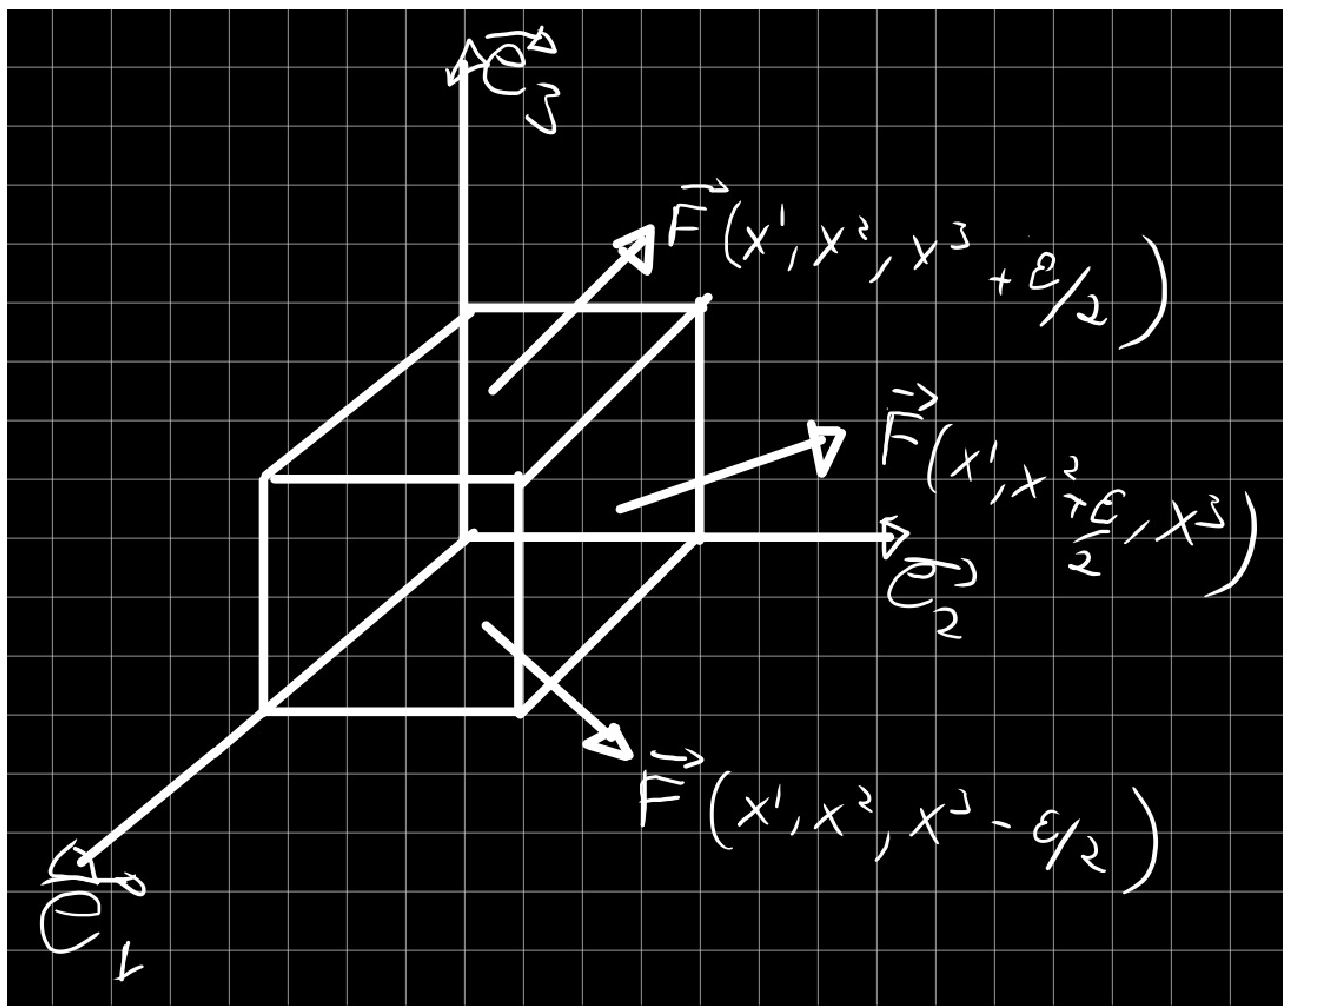
\includegraphics[scale=0.5]{Div.pdf} \caption{Campo vetorial ao redor
		de um cubo de lado $\varepsilon$, centrado em $\vec{x}$. Dado com campo vetorial
		$\vec{F}(\vec{x})$ e um cubo centrado em $\vec{x}$ temos, por exemplo, que o
		campo no centro face superior é $\vec{F}(x^1,x^2,x^3+\varepsilon/2)$.
		\label{fig:div}}
\end{figure}

Dado um campo vetorial $\vec{F}$ podemos calcular o fluxo total do campo em um
certo ponto $\vec{x}$. Para tanto precisamos calcular a projeção do campo nas
direções externas a um ponto. Fazemos isso considerando um cubo de lado
$\varepsilon$ centrado em $\vec{x}$ como mostrado na Fig.~\ref{fig:div}. Os
vetores ortogonais as faces superior e inferior são respectivamente $\vec{e}_3$
e $-\vec{e}_3$, de forma similar os pares $\vec{e}_1$, $-\vec{e}_1$ e $\vec{e}_2$,
$-\vec{e}_2$ são ortogonais as outras quatro faces. Suponha que o cubo é pequeno
suficiente, de forma que podemos aproximar o fluxo por uma face, a face superior
por exemplo, por $\vec{F}(x^1, x^2, x^3 + \varepsilon/2) \cdot
	\left(\varepsilon^2 \vec{e}_3\right)$, onde $\varepsilon^2\vec{e}_3$ representa
a área de face e a direção perpendicular a ela. Assim, o fluxo total para fora
desse objeto é dados pelas some dos fluxos pelas faces dividida pelo volume
total, ou divergente, é dado por
\begin{equation}\label{limdiv}
	\begin{split}
		\mathrm{div}(\vec{F}) = \lim_{\varepsilon\to0}\frac{1}{\varepsilon^3}\Big[ & \vec{F}(x^1,x^2,x^3+\varepsilon/2)\cdot\left(\varepsilon^2\vec{e}_3\right)+\vec{F}(x^1,x^2,x^3-\varepsilon/2)\cdot\left(-\varepsilon^2\vec{e}_3\right) +     \\
		                                                                           & \vec{F}(x^1,x^2+\varepsilon/2,x^3)\cdot\left(\varepsilon^2\vec{e}_2\right)+\vec{F}(x^1,x^2-\varepsilon/2,x^3)\cdot\left(-\varepsilon^2\vec{e}_2\right) +     \\
		                                                                           & \vec{F}(x^1+\varepsilon/2,x^2,x^3)\cdot\left(\varepsilon^2\vec{e}_1\right)+\vec{F}(x^1-\varepsilon/2,x^2,x^3)\cdot\left(-\varepsilon^2\vec{e}_1\right)\Big].
	\end{split}
\end{equation}
Calculando a série de Maclaurin e tomando o limite podemos mostrar facilmente que
\begin{equation}
	\mathrm{div}(\vec{F}) = \sum_{i=1}^3\frac{\partial F^i}{\partial x^i}(\vec{x}) = \nabla\cdot\vec{F}(\vec{x}).
\end{equation}
Lembre-se que estramos usando vetores coordenados $\vec{x}$, caso contrário os
produtos escalares utilizados não teriam o significado geométrico correto. O
operador $\nabla$ pode portanto ser usado para calcular o divergente de um campo
vetorial tomando seu produto interno entre esses dois objetos.

\begin{figure}
	\centering 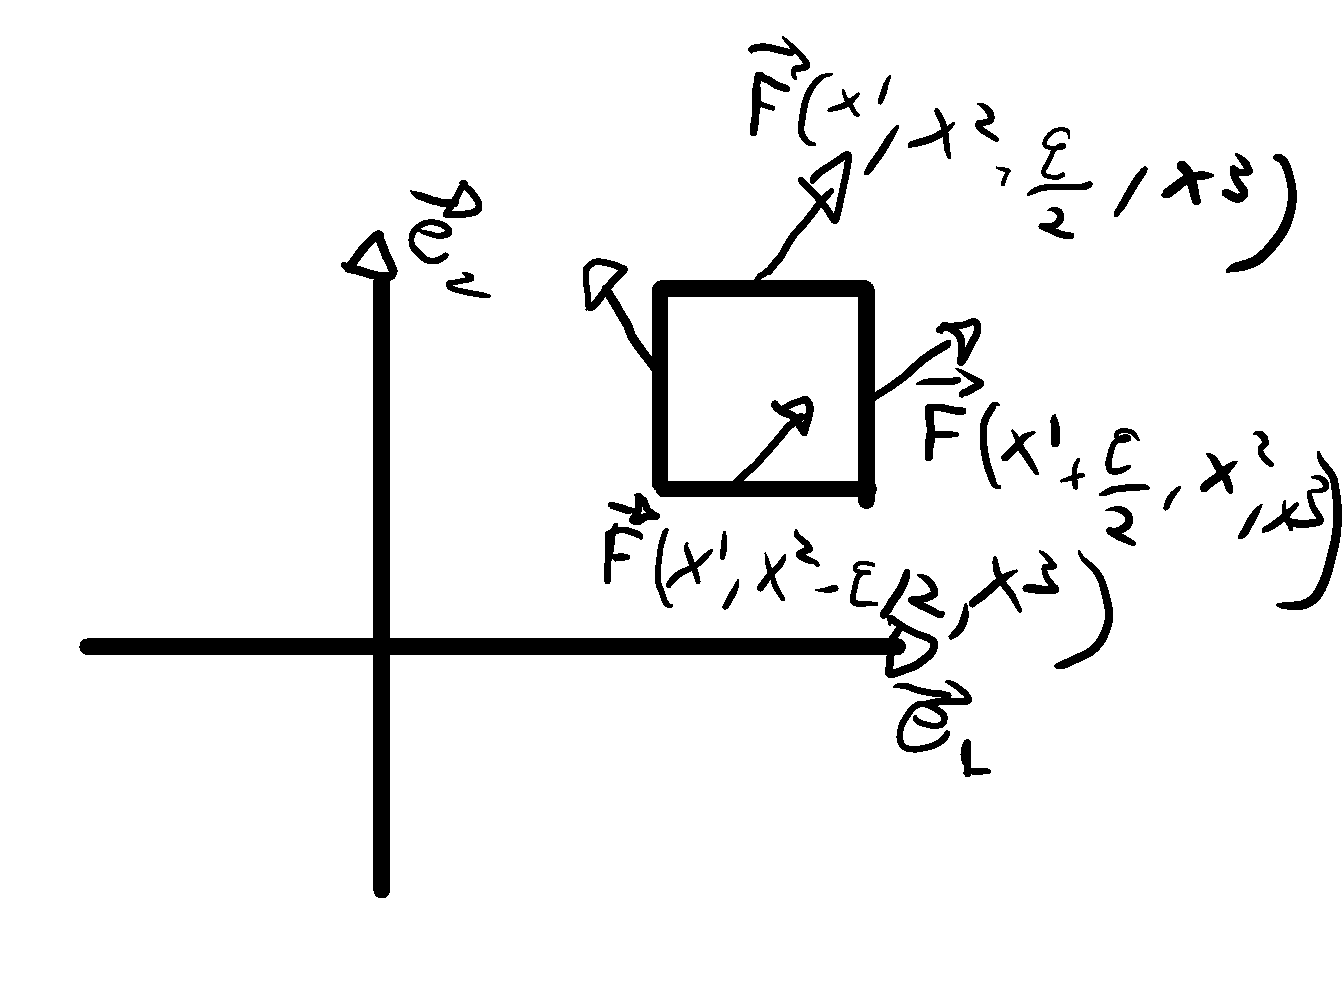
\includegraphics[scale=0.5]{Rot.pdf}
	\caption{Campo vetorial ao de uma circuito quadrado de lado $\varepsilon$,
		centrado em $\vec{x}$.\label{fig:rot}}
\end{figure}

\subsection{Rotacional}
\label{sec:rot}

Outra quantidade de interesse que podemos extrair de um campo vetorial é a sua circulação em torno de um ponto. Considere a Fig.~\ref{fig:rot}, lá temos um circuito quadrado e um campo vetorial de exemplo. Convencionando o sentido anti-horário, podemos calcular o rotacional do campo nesse plano, isto é, a circulação nesse circuito dividida pela área compreendida por ele, para tanto calculamos a projeção de $\vec{F}(x^1+\varepsilon/2, x^2,x^3)$ na direção $\varepsilon\vec{e}_2$, a projeção de $\vec{F}(x^1, x^2+\varepsilon/2,x^3)$ na direção $-\varepsilon\vec{e}_1$, e assim por diante, ou seja,
\begin{equation}\label{limrot}
	\begin{split}
		\mathrm{rot}(\vec{F})_{\vec{e}_1\wedge\vec{e}_2} =\lim_{\varepsilon\to0}\frac{1}{\varepsilon^2}\Big[ & \vec{F}(x^1+\varepsilon/2, x^2,x^3)\cdot\left(\varepsilon\vec{e}_2\right) + \vec{F}(x^1-\varepsilon/2, x^2,x^3)\cdot\left(-\varepsilon\vec{e}_2\right)        \\
		                                                                                                     & +\vec{F}(x^1, x^2+\varepsilon/2,x^3)\cdot\left(-\varepsilon\vec{e}_1\right) + \vec{F}(x^1, x^2-\varepsilon/2,x^3)\cdot\left(\varepsilon\vec{e}_1\right)\Big].
	\end{split}
\end{equation}
Novamente, calculamos a série de Maclaurin e tomamos o limite e encontramos
\begin{equation}
	\mathrm{rot}(\vec{F})_{\vec{e}_1\wedge\vec{e}_2} = \frac{\partial F^2(\vec{x})}{\partial x^1} - \frac{\partial F^1(\vec{x})}{\partial x^2}.
\end{equation}
De forma análoga, podemos calcular a circulação nos outros dois plano,
\begin{align}
	\mathrm{rot}(\vec{F})_{\vec{e}_1\wedge\vec{e}_3} & = \frac{\partial F^3(\vec{x})}{\partial x^1} - \frac{\partial F^1(\vec{x})}{\partial x^3}, \\
	\mathrm{rot}(\vec{F})_{\vec{e}_2\wedge\vec{e}_3} & = \frac{\partial F^3(\vec{x})}{\partial x^2} - \frac{\partial F^2(\vec{x})}{\partial x^3}.
\end{align}
A aplicação do produto externo entre o operador $\nabla$ e o campo $\vec{F}$, tem o seguinte resultado,
\begin{equation}
	\nabla\wedge\vec{F} = \left[\frac{\partial F^2}{\partial x^1} - \frac{\partial F^1}{\partial x^2}\right]\vec{e}_1\wedge\vec{e}_2+\left[\frac{\partial F^3}{\partial x^1} - \frac{\partial F^1}{\partial x^3}\right]\vec{e}_1\wedge\vec{e}_3+\left[\frac{\partial F^3}{\partial x^2} - \frac{\partial F^2}{\partial x^3}\right]\vec{e}_2\wedge\vec{e}_3,
\end{equation}
onde, por simplicidade, omitimos os argumentos $(\vec{x})$ das funções.
Aplicando nosso operador $V$ temos o resultado em termos do produto vetorial,
\begin{equation}
	\nabla\times\vec{F} = \left[\frac{\partial F^2}{\partial x^1} - \frac{\partial F^1}{\partial x^2}\right]\vec{e}_3-\left[\frac{\partial F^3}{\partial x^1} - \frac{\partial F^1}{\partial x^3}\right]\vec{e}_2+\left[\frac{\partial F^3}{\partial x^2} - \frac{\partial F^2}{\partial x^3}\right]\vec{e}_1.
\end{equation}
Portanto, o rotacional calculado usando o produto vetorial retorna um campo
pseudo-vetorial cujas componentes contêm o valor da circulação do campo no plano
perpendicular a direção da componente.

\subsection{Derivadas segundas}

Usando as regras de produtos triplos derivadas nas seções anteriores, podemos
facilmente calcular todas as derivadas segundas compondo diferentes aplicações
do operador $\nabla$. Vale ressaltar que além das regras de composição dos
produtos, é necessário lembrar que as derivadas satisfazem a regra de Leibniz
quando age sobre produto de funções, por exemplo,
\begin{align}
	\label{leibniz1} \nabla\left[f(\vec{x})g(\vec{x})\right]                        & = g(\vec{x})\nabla f(\vec{x})+f(\vec{x})\nabla g(\vec{x}),                                                                        & f(\vec{x}), g(\vec{x}) & \in C^\infty(\mathbb{R}^3), \\
	\nabla\cdot\left[f(\vec{x})\vec{F}(\vec{x})\right]                              & = \nabla f(\vec{x})\cdot\vec{F}(\vec{x}) + f(\vec{x})\nabla \cdot\vec{F}(\vec{x}),                                                & \vec{F}(\vec{x})       & \in \mathbb{V},             \\
	\nabla\times\left[f(\vec{x})\vec{F}(\vec{x})\right]                             & = \nabla f(\vec{x})\times\vec{F}(\vec{x}) + f(\vec{x})\nabla \times\vec{F}(\vec{x}),                                                                                                     \\
	\label{leibnizl} \nabla\cdot\left[\vec{F}(\vec{x})\times\vec{G}(\vec{x})\right] & = \vec{G}(\vec{x})\cdot\left[\nabla\times\vec{F}(\vec{x})\right] - \vec{F}(\vec{x})\cdot\left[\nabla\times\vec{G}(\vec{x})\right] & \vec{G}(\vec{x})       & \in \mathbb{V},             \\
	\label{leibnizf}\nabla\times\left[\vec{F}(\vec{x})\times\vec{G}(\vec{x})\right] & = \left[\nabla\cdot\vec{G}(\vec{x})\right]\vec{F}(\vec{x}) + \left[\vec{G}(\vec{x})\cdot\nabla\right]\vec{F}(\vec{x})                                                                    \\
	                                                                                & - \left[\nabla\cdot\vec{F}(\vec{x})\right]\vec{G}(\vec{x}) - \left[\vec{F}(\vec{x})\cdot\nabla\right]\vec{G}(\vec{x}).
\end{align}

Uma das derivadas segundas que aparecem com grande frequência em aplicações
físicas é o operador Laplaciano.
\definition{Laplaciano $\nabla^2$ é o resultado da aplicação do gradiente
	seguido de sua divergência, ou seja,
	\begin{equation}\label{LBo}
		\nabla^2f(\vec{x}) \equiv \nabla\cdot\nabla f(\vec{x}).
	\end{equation}
	Note que esse é um operador escalar, leva uma função em uma função, ou um vetor
	em um vetor. }

As outras derivadas segundas podem ser facilmente deduzidas utilizando as regras de composição de operações, assim como utilizamos nas Eqs.~\eqref{leibniz1}--\eqref{leibnizf}.

\begin{Exercise}[title={Cálculo diferencial}]
	\Question[difficulty=1] Calcular explicitamente a série e o limite nas
	Eqs.~\eqref{limgrad}, \eqref{limdiv} e \eqref{limrot}.
	\Question Calcular o divergente do gradiente de uma função de $f(\vec{x}) \in C^\infty(\mathbb{R}^3)$.
	\Question Calcular o rotacional de um gradiente de uma função de $f(\vec{x}) \in C^\infty(\mathbb{R}^3)$.
	\Question Provar as Eqs.~\eqref{leibniz1}--\eqref{leibnizf}. Dica: use Eq.~\eqref{VandUv} para mostrar Eq.~\eqref{leibnizl}; Equação~\eqref{leibnizf} pode ser obtida diretamente da Eq.~\eqref{vprod2} usando a regra de Leibniz.
\end{Exercise}

\section{Cálculo integral}
\label{sec:int}
\subsection{Integração em uma dimensão}

O teorema fundamental do cálculo relaciona a integral definida de uma função com
a avaliação da sua antiderivada nos extremos de integração, i.e.,
\begin{equation}\label{intdef}
	\int_a^b\frac{\dd f(x)}{\dd x}\dd x  = f(b) - f(a), \quad a,b\in\mathbb{R}, \quad f:\mathbb{R}\to\mathbb{R}.
\end{equation}
É interessante destacar o que a equação acima significa. A integral da derivada
de uma função em um intervalo $(a, b)$ é igual ao valor da própria função
avaliada nos extremos. Note que os extremos do intervalo fazem o papel da
hipersuperfície de dimensão zero que circunda o intervalo. Existem portanto uma
relação próxima entre a geometria do intervalo que está sendo integrado, a
hipersuperfície que o cerca e o integrando. Vamos ver nas seções seguintes que
essa estrutura se mantem quando passamos para integrais em mais dimensões.

\subsection{Integral de linha}
\label{sec:intline}

A primeira generalização que podemos fazer da integração unidimensional é a
integral de linha. Dada um campo vetorial $\vec{F}(\vec{x})$ e uma curva
$\mathcal{C}$ parametrizada por $\vec{c}:\mathrm{R}\to\mathrm{R}^3$ que dado o
valor do seu parâmetro $\lambda\in\mathbb{R}$ nos dá um ponto
$\vec{c}(\lambda) \in \mathbb{R}^3$, a integral de $\vec{F}$ sob essa curva é:
\begin{equation}
	\int_\mathcal{C}\vec{F}\cdot\dd \vec{c} \equiv  \int_{\lambda_0}^{\lambda_1}\vec{F}(\vec{c}(\lambda))\cdot \dot{\vec{c}}(\lambda)\dd \lambda, \qquad \dot{\vec{c}}(\lambda) \equiv \frac{\dd \vec{c}(\lambda)}{\dd \lambda}.
\end{equation}
Em palavras, a integral acima calcula a soma das projeções de $\vec{F}$ na
direção da variação da curva $\dot{\vec{c}}$ em cada ponto da curva. Novamente,
chamamos atenção ao fato de que nosso produto interno tem significado geométrico
em coordenadas cartesianas e portanto $\dot{\vec{c}}$ e $\vec{F}$ são vetores no
espaço tangente em coordenadas cartesianas.

Para obtermos uma expressão similar a~\eqref{intdef}, precisamos da integral de
uma derivada, nesse caso é fácil notar que se $\vec{F}(\vec{x}) = \nabla f(\vec{x})$
para $f(\vec{x}) \in C^{\infty}(\mathbb{R}^3)$, temos
\begin{equation}
	\int_{\lambda_0}^{\lambda_1}\nabla f(\vec{c}(\lambda))\cdot \dot{\vec{c}}(\lambda)\dd \lambda = \int_{\lambda_0}^{\lambda_1}\frac{\dd }{\dd \lambda}\left[f(\vec{c}(\lambda))\right]\dd \lambda = f(\vec{c}(\lambda_1)) - f(\vec{c}(\lambda_0)).
\end{equation}
Essa expressão é exatamente análoga a Eq.~\eqref{intdef}, inclusive utilizamos
essa equação para passar do segundo para o terceiro termo. Dado o resultado
acima, é fácil ver que se a curva for fechada, $\vec{c}(\lambda_1) =
	\vec{c}(\lambda_0)$, a integral é zero. De qualquer forma, toda informação da
integral está novamente contida na hipersuperfície que cobre a curva (nesse caso
suas pontas).

\subsection{Integral de superfície}

O próximo passo é calcular integrais de superfície. Para tanto, começamos por
definir a superfície e o elemento de área. Uma superfície em $\mathbb{R}^3$ pode
ser parametrizada por um vetor $\vec{S}(\lambda,\mu)$ de forma que ao variar
$\lambda \in (\lambda_0,\,\lambda_1)$ e $\mu \in (\mu_0,\,\mu_1)$ o vetor
$\vec{S}(\lambda,\mu)$ percorre toda a superfície, que chamaremos de
$\mathcal{S}$. Usando esse vetor, podemos cacular vetores tangentes a essas
curvas calculando sua derivada em relação aos parâmetros $(\lambda,\mu)$, i.e.,
\begin{equation}\label{def:S}
	\vec{S}_\lambda(\lambda,\mu) \equiv \frac{\partial \vec{S}(\lambda,\mu)}{\partial\lambda}, \qquad \vec{S}_\mu(\lambda,\mu) \equiv \frac{\partial \vec{S}(\lambda,\mu)}{\partial\mu}.
\end{equation}
Como vimos na Sec.~\ref{sec:eprod} o produto externo (e o produto vetorial)
de dois vetores tem como modulo a área do paralelogramo definido por eles,
assim, a área infinitesimal é dada por
\begin{equation}
	\dd A \equiv \vec{S}_\lambda(\lambda,\mu)\wedge\vec{S}_\mu(\lambda,\mu)\dd \lambda\dd \mu \quad\text{ou}\quad \dd \vec{a} \equiv \vec{S}_\lambda(\lambda,\mu)\times\vec{S}_\mu(\lambda,\mu)\dd \lambda\dd \mu.
\end{equation}
Note que esse elemento fornece a área e também uma direção, portanto para fazer
integrais de superfície é necessário também definir a orientação da superfície.

Com o elemento de área em mãos, definimos a integral de superfície do campo
vetorial $\vec{F}(\vec{x})$ na projetado na direção perpendicular as áreas por
\begin{equation}\label{intsurf}
	\int_{\mathcal{S}} \dd \vec{a}\cdot \vec{F}(\vec{S}(\lambda,\mu)) = \int_{\lambda_0}^{\lambda_1}\dd \lambda\int_{\mu_0}^{\mu_1}\dd \mu \left[\vec{S}_\lambda(\lambda,\mu)\times\vec{S}_\mu(\lambda,\mu)\right]\cdot \vec{F}(\vec{S}(\lambda,\mu)).
\end{equation}
Como vimos  na Sec.~\ref{sec:rot} o rotacional de um campo projetado em uma
certa direção $\vec{u}$ nos dá a circulação dele em relação a área ortogonal a
$\vec{u}$. Dessa forma, se na integral acima o campo for o resultado de um
rotacional $\vec{F}(\vec{x}) = \nabla\times\vec{v}(\vec{x})$ (onde
$\vec{v}(\vec{x})$ é um campo vetorial), a integral de superfície nos fornecerá
o valor da circulação do campo na área integrada $\mathcal{S}$, isto é,
\begin{equation}
	\int_{\mathcal{S}} \dd \vec{a}\cdot \left[\nabla\times\vec{v}\left(\vec{S}(\lambda,\mu)\right)\right] =  \int_{\lambda_0}^{\lambda_1}\dd \lambda\int_{\mu_0}^{\mu_1}\dd \mu \left[\vec{S}_\lambda(\lambda,\mu)\times\vec{S}_\mu(\lambda,\mu)\right]\cdot\left[\nabla\times\vec{v}\left(\vec{S}(\lambda,\mu)\right)\right].
\end{equation}
Na integral do lado direito temos um produto interno de dois produtos vetoriais,
portanto para simplificar a expressão acima, vamos primeiro calcular o produto
(onde vamos omitir os argumentos das funções por simplicidade)
\begin{align}
	\left(\vec{S}_\lambda\times\vec{S}_\mu\right)\cdot\left(\nabla\times\vec{v}\right) & = \Upsilon\left[V\left(\nabla\wedge\vec{v}\right)\wedge\vec{S}_\lambda\wedge\vec{S}_\mu\right],                                   \\
	                                                                                   & =\Upsilon\left(V^{-1}\left\{V\left[V\left(\nabla\wedge\vec{v}\right)\wedge\vec{S}_\lambda\right]\right\}\wedge\vec{S}_\mu\right),
\end{align}
onde usamos Eq.~\eqref{VandUv} para escrever a primeira igualdade e introduzimos
um operador identidade $V^{-1}(V(\dots))$. O termo de dentro das chaves pode ser
expressado como
\begin{equation}
	V\left[V\left(\nabla\wedge\vec{v}\right)\wedge\vec{S}_\lambda\right] = (\vec{S}_\lambda\cdot\nabla)\vec{v} - \sum_{i=1}^3\vec{e}_i\left[\left(\frac{\partial \vec{v}}{\partial x^i}\right)\cdot\vec{S}_\lambda\right],
\end{equation}
onde usamos agora a Eq.~\eqref{vprod2}. Finalmente, podemos aplicar o
resultado~\eqref{UVm1} e obter
\begin{equation}
	\left(\vec{S}_\lambda\times\vec{S}_\mu\right)\cdot\left(\nabla\times\vec{v}\right) = \vec{S}_\mu\cdot\left[\left(\vec{S}_\lambda\cdot\nabla\right)\vec{v}\right] - \vec{S}_\lambda\cdot\left[\left(\vec{S}_\mu\cdot\nabla\right)\vec{v}\right].
\end{equation}
Lembrando agora que todos os campos vetoriais estão avaliados em
$\vec{S}(\lambda,\mu)$, temos que os termos nos colchetes são derivadas totais
de $\vec{v}$ em relação a $\lambda$ e $\mu$ respectivamente, ou seja,
\begin{align}
	\left(\vec{S}_\lambda\times\vec{S}_\mu\right)\cdot\left(\nabla\times\vec{v}\right) & = \vec{S}_\mu(\lambda,\mu)\cdot\left[\frac{\dd \vec{v}(\vec{S}(\lambda,\mu))}{\dd \lambda}\right] - \vec{S}_\lambda(\lambda,\mu)\cdot\left[\frac{\dd \vec{v}(\vec{S}(\lambda,\mu))}{\dd \mu}\right], \\
	\nonumber                                                                          & =\frac{\dd }{\dd \lambda}\left[\vec{S}_\mu\cdot\vec{v}(\vec{S}(\lambda,\mu))\right] - \frac{\dd }{\dd \mu}\left[\vec{S}_\lambda\cdot\vec{v}(\vec{S}(\lambda,\mu))\right]                             \\
	                                                                                   & -\vec{v}(\vec{S}(\lambda,\mu))\cdot\left[\frac{\dd \vec{S}_\mu(\lambda,\mu)}{\dd \lambda}-\frac{\dd \vec{S}_\lambda(\lambda,\mu)}{\dd \mu}\right].
\end{align}
Veja que o último termo da expressão acima é zero devido a comutação das
derivadas parciais (veja Eq.~\eqref{def:S}), assim temos então
\begin{equation}
	\int_{\mathcal{S}} \dd \vec{a}\cdot \left[\nabla\times\vec{v}\left(\vec{S}(\lambda,\mu)\right)\right] = \int_{\mu_0}^{\mu_1}\dd \mu\left[\vec{S}_\mu\cdot\vec{v}(\vec{S}(\lambda,\mu))\right]_{\lambda_0}^{\lambda_1} - \int_{\lambda_0}^{\lambda_1}\dd \lambda\left[\vec{S}_\lambda\cdot\vec{v}(\vec{S}(\lambda,\mu))\right]_{\mu_0}^{\mu_1}.
\end{equation}
As integrais do lado direito da expressão acima são simplesmente a integral de
linha do campo $\vec{v}(\vec{x})$ projetado na direção das bordas (considerando
o sentido horário) do quadrado definido por $(\lambda_0, \lambda_1) \times
	(\mu_0, \mu_1)$. Usando o símbolo $\partial\mathcal{S}$ para denotar a borda de
$\mathcal{S}$, podemos escrever o lado direito usando a notação da
Sec.~\ref{sec:intline},
\begin{equation}\label{stokes}
	\int_{\mathcal{S}} \dd \vec{a}\cdot \left(\nabla\times\vec{v}\right) = \int_{\partial\mathcal{S}}\vec{v}\cdot\dd \vec{c}.
\end{equation}
onde $\vec{c}$ é o vetor tangente a curva descrita por $\vec{S}_\lambda$ e
$\vec{S}_\mu$ avaliados nas bordas do quadrado $(\lambda_0, \lambda_1) \times
	(\mu_0, \mu_1)$.

A Eq.~\eqref{stokes} é conhecida como teorema de Stokes, nesse caso a integral
de uma superfície está relacionada à integral de sua borda. Aqui vemos mais
claramente que esses resultados relacionam uma integral em $n$ dimensões com uma
integral em $n-1$.

\subsection{Integral de volume}
\label{sec:intvol}

Por fim, podemos calcular integrais de um campo vetoriais em volumes. Para tanto
note que o elemento de integração agora não é mais um vetor. Como vimos na
Sec.~\ref{sec:trip} o produto triplo~\eqref{VandUv} resulta no volume do
paralelepípedo formado por três vetores linearmente independentes. De forma
similar ao que fizemos no caso das superfícies, seja $\vec{x}(\lambda,\mu,\nu)$
um vetor parametrizado por
$$(\lambda,\mu,\nu) \in (\lambda_0,\lambda_1)\times(\mu_0,\mu_1)\times(\nu_0,\mu_1) \subset \mathbb{R}^3.$$
de forma que ao variar os parâmetros nesses intervalo, o vetor $
	\vec{x}(\lambda,\mu,\nu) $ percorre todo o volume $\mathcal{V}$. Os vetores
associados a pequenas variações em cada um dos parâmetros são:
\begin{equation}
	\vec{x}_\lambda(\lambda,\mu,\nu) \equiv \frac{\partial\vec{x}(\lambda,\mu,\nu)}{\partial\lambda}, \quad
	\vec{x}_\mu(\lambda,\mu,\nu) \equiv \frac{\partial\vec{x}(\lambda,\mu,\nu)}{\partial\mu}, \quad
	\vec{x}_\nu(\lambda,\mu,\nu) \equiv \frac{\partial\vec{x}(\lambda,\mu,\nu)}{\partial\nu}.
\end{equation}
Assim, o volume do paralelepípedo formado por essas pequenas variações é
\begin{equation}
	\dd \vec{x} \equiv \Upsilon\left(\vec{x}_\lambda\wedge\vec{x}_\mu\wedge\vec{x}_\nu\right)\dd \lambda\,\dd \mu\,\dd \nu,
\end{equation}
onde omitimos o argumento $(\lambda,\mu,\nu)$ dos vetores por simplicidade.
Portanto, a integral de uma função escalar $f\in C^{\infty}(\mathbb{R}^3)$ no
volume $\mathcal{V}$ é dada por
\begin{equation}
	\int_{\mathcal{V}}f \dd \vec{x} = \int_{\lambda_0}^{\lambda_1}\dd \lambda\int_{\mu_0}^{\mu_1}\dd \mu\int_{\nu_0}^{\nu_1}\dd \nu\, \Upsilon\left(\vec{x}_\lambda(\lambda,\mu,\nu)\wedge\vec{x}_\mu(\lambda,\mu,\nu)\wedge\vec{x}_\nu(\lambda,\mu,\nu)\right)f\left(\vec{x}(\lambda,\mu,\nu)\right).
\end{equation}
Na Sec.~\ref{sec:div} vimos que o divergente de um campo nos da o fluxo do campo
passando por um ponto. Dessa forma, se nossa função escalar integrada no volume
$\mathcal{V}$ for um divergente, a integral resultará no fluxo total
entrando/saindo de $\mathcal{V}$. Em outras palavras, dado $f =
	\nabla\cdot\vec{F}$ para um campo vetorial $\vec{F}(\vec{x})$, temos
\begin{equation*}
	\int_{\mathcal{V}}\nabla\cdot\vec{F}\, \dd \vec{x} = \int_{\lambda_0}^{\lambda_1}\dd \lambda\int_{\mu_0}^{\mu_1}\dd \mu\int_{\nu_0}^{\nu_1}\dd \nu\, \Upsilon\left(\vec{x}_\lambda\wedge\vec{x}_\mu\wedge\vec{x}_\nu\right)\nabla\cdot\vec{F},
\end{equation*}
omitindo os argumentos $(\lambda,\mu,\nu)$ para obter expressões mais compactas,
continuaremos essa omissão até o fim da seção. Como o operador $\Upsilon$ é
linear, podemos colocar o divergente (que é um escalar) dentro do operador, ou
seja,
\begin{equation}
	\int_{\mathcal{V}}\nabla\cdot\vec{F}\, \dd \vec{x} = \int_{\lambda_0}^{\lambda_1}\dd \lambda\int_{\mu_0}^{\mu_1}\dd \mu\int_{\nu_0}^{\nu_1}\dd \nu\, \Upsilon\left(\vec{x}_\lambda\wedge\vec{x}_\mu\wedge\vec{x}_\nu\,\nabla\cdot\vec{F}\right),
\end{equation}
usando a Eq.~\eqref{intdet} podemos reescrever o termo dentro dos parênteses do
lado direito da expressão acima como
\begin{equation}\label{prepp}
	\vec{x}_\lambda\wedge\vec{x}_\mu\wedge\vec{x}_\nu\,\nabla\cdot\vec{F} =\left(\vec{x}_\lambda\cdot\nabla\vec{F}\right)\wedge\vec{x}_\mu\wedge\vec{x}_\nu-\left(\vec{x}_\mu\cdot\nabla\vec{F}\right)\wedge\vec{x}_\lambda\wedge\vec{x}_\nu+\left(\vec{x}_\nu\cdot\nabla\vec{F}\right)\wedge\vec{x}_\lambda\wedge\vec{x}_\mu,
\end{equation}
os termos entre parênteses no lado direito da última expressão são simplesmente
as derivadas totais de $\vec{F}\left(\vec{x}(\lambda,\mu,\nu)\right)$ em relação
a $\lambda$, $\mu$ e $\nu$ respectivamente, isto é,
\begin{equation}\label{semi1}
	\vec{x}_\lambda\wedge\vec{x}_\mu\wedge\vec{x}_\nu\,\nabla\cdot\vec{F} = \left[\frac{\dd \vec{F}\left(\vec{x}\right)}{\dd \lambda}\right]\wedge\vec{x}_\mu\wedge\vec{x}_\nu-\left[\frac{\dd \vec{F}\left(\vec{x}\right)}{\dd \mu}\right]\wedge\vec{x}_\lambda\wedge\vec{x}_\nu +\left[\frac{\dd \vec{F}\left(\vec{x}\right)}{\dd \nu}\right]\wedge\vec{x}_\lambda\wedge\vec{x}_\mu.
\end{equation}
Cada um dos termos do lado direito pode ser escrito como uma derivada total
menos um termo com a mesma derivada atuando no resto da expressão, por exemplo,
o primeiro termo fica
\begin{align*}
	\left[\frac{\dd \vec{F}\left(\vec{x}\right)}{\dd \lambda}\right]\wedge\vec{x}_\mu\wedge\vec{x}_\nu = \frac{\dd }{\dd \lambda}\left[\vec{F}\left(\vec{x}\right)\wedge\vec{x}_\mu\wedge\vec{x}_\nu\right] - \vec{F}\left(\vec{x}\right)\wedge\frac{\partial}{\partial\lambda}\left[\vec{x}_\mu\wedge\vec{x}_\nu\right]. \end{align*}
Usando esse resultado, reescrevemos a Eq.~\eqref{semi1} da forma
\begin{equation}\label{pospp}
	\vec{x}_\lambda\wedge\vec{x}_\mu\wedge\vec{x}_\nu\,\nabla\cdot\vec{F} = \frac{\dd }{\dd \lambda}\left[\vec{F}\left(\vec{x}\right)\wedge\vec{x}_\mu\wedge\vec{x}_\nu\right]
	-\frac{\dd }{\dd \mu}\left[\vec{F}\left(\vec{x}\right)\wedge\vec{x}_\lambda\wedge\vec{x}_\nu\right]
	+\frac{\dd }{\dd \nu}\left[\vec{F}\left(\vec{x}\right)\wedge\vec{x}_\lambda\wedge\vec{x}_\mu\right],
\end{equation}
onde os outros três termos se cancelam devido a comutação das derivadas
parciais. Veja que a dedução acima reduz o integrando de nossa integral de
volume a soma de três termos de derivadas totais. Assim, nossa expressão inicial
fica simplificada na forma
\begin{equation}
	\begin{split}
		\int_{\mathcal{V}}\nabla\cdot\vec{F}\, \dd \vec{x} & = \int_{\mu_0}^{\mu_1}\dd \mu\int_{\nu_0}^{\nu_1}\dd \nu\, \Upsilon\left(
		\left[\vec{F}\left(\vec{x}\right)\wedge\vec{x}_\mu\wedge\vec{x}_\nu\right]_{\lambda_0}^{\lambda_1}
		\right)                                                                                                                                                                                                                                 \\
		                                                   & -\int_{\lambda_0}^{\lambda_1}\dd \lambda\int_{\nu_0}^{\nu_1}\dd \nu\, \Upsilon\left(
		\left[\vec{F}\left(\vec{x}\right)\wedge\vec{x}_\lambda\wedge\vec{x}_\nu\right]_{\mu_0}^{\mu_1}
		\right)                                                                                                                                                                                                                                 \\
		                                                   & +\int_{\lambda_0}^{\lambda_1}\dd \lambda\int_{\mu_0}^{\mu_1}\dd \mu\, \Upsilon\left(\left[\vec{F}\left(\vec{x}\right)\wedge\vec{x}_\lambda\wedge\vec{x}_\mu\right]_{\nu_0}^{\nu_1}
		\right),
	\end{split}
\end{equation}
o que mostra que nossa integral no volume se reduz as integrais na superfície do
cubo $(\lambda_0,\lambda_1)\times(\mu_0,\mu_1)\times(\nu_0,\mu_1)$. Para deixar
esse resultado em uma forma mais familiar, usamos a Eq.~\eqref{UVm1} para
reescrever as projeções $\Upsilon$ usando, por exemplo,
$$\Upsilon\left(\vec{F}\left(\vec{x}\right)\wedge\vec{x}_\mu\wedge\vec{x}_\nu\right) = \vec{F}\left(\vec{x}\right)\cdot\left(\vec{x}_\mu\times\vec{x}_\nu\right),$$
para mostrar que
\begin{equation}\label{pregauss}
	\begin{split}
		\int_{\mathcal{V}}\nabla\cdot\vec{F}\, \dd \vec{x} & = \int_{\mu_0}^{\mu_1}\dd \mu\int_{\nu_0}^{\nu_1}\dd \nu\,
		\left[\vec{F}\left(\vec{x}\right)\cdot\left(\vec{x}_\mu\times\vec{x}_\nu\right)\right]_{\lambda_0}^{\lambda_1}
		-\int_{\lambda_0}^{\lambda_1}\dd \lambda\int_{\nu_0}^{\nu_1}\dd \nu\,
		\left[\vec{F}\left(\vec{x}\right)\cdot\left(\vec{x}_\lambda\times\vec{x}_\nu\right)\right]_{\mu_0}^{\mu_1}                                                                                                                             \\
		                                                   & +\int_{\lambda_0}^{\lambda_1}\dd \lambda\int_{\mu_0}^{\mu_1}\dd \mu\, \left[\vec{F}\left(\vec{x}\right)\cdot\left(\vec{x}_\lambda\times\vec{x}_\mu\right)\right]_{\nu_0}^{\nu_1},
	\end{split}
\end{equation}
Comparando cada termo da expressão acima, vemos que os termos da direita
representam a integral na superfície de $\mathcal{V}$ que denotamos por
$\partial\mathcal{V}$, e os vetores ortogonais as superfícies por $\vec{S}$,
então finalmente temos
\begin{equation}
	\int_{\mathcal{V}}\nabla\cdot\vec{F}\, \dd \vec{x} = \int_{\partial\mathcal{V}}\vec{F}\cdot \dd \vec{S}.
\end{equation}
Essa expressão é conhecida como teorema da divergência ou teorema de Gauss.

\example{\label{ex:spher} Se quisermos fazer a integral em uma esfera de raio $R$, podemos
	facilmente encontrar o vetor $\vec{x}$ como função das coordenadas esféricas
	$(r,\theta,\varphi) \in (0,R)\times(0,\pi)\times(0,2\pi)$ (que aqui fazem o
	papel de $(\lambda,\mu,\nu)$).
	\begin{equation}
		\vec{x}(r,\theta,\varphi) = r \sin\theta\cos\phi\,\vec{e}_1+r \sin\theta\sin\phi\,\vec{e}_2+r \cos\theta\,\vec{e}_3.
	\end{equation}
	Nessas coordenadas temos
	\begin{align}
		\vec{e}_r       & \equiv \frac{\partial \vec{x}}{\partial r}= \sin\theta\cos\varphi\,\vec{e}_1+\sin\theta\sin\varphi\,\vec{e}_2+\cos\theta\,\vec{e}_3,         \\
		\vec{e}_\theta  & \equiv \frac{\partial \vec{x}}{\partial \theta}= r\cos\theta\cos\varphi\,\vec{e}_1+r\cos\theta\sin\varphi\,\vec{e}_2-r\sin\theta\,\vec{e}_3, \\
		\vec{e}_\varphi & \equiv \frac{\partial \vec{x}}{\partial \varpi}= -r\sin\theta\sin\varphi\,\vec{e}_1+r\sin\theta\cos\varphi\,\vec{e}_2.
	\end{align}
	Fazendo a conta direta podemos mostrar que
	\begin{align}
		\vec{e}_r\times \vec{e}_\theta       & = -r \sin\theta\,\vec{e}_1+r\cos\theta\,\vec{e}_2, \\
		\vec{e}_r\times \vec{e}_\varphi      & = -\sin\theta\,\vec{e}_\theta,                     \\
		\vec{e}_\theta\times \vec{e}_\varphi & = r^2\sin\theta\,\vec{e}_r.
	\end{align}
	Quando usamos esses resultados na Eq.~\eqref{pregauss} notamos que o termo
	integrado em $r$ em $(0,R)$, somente o termo no extremo $R$ é diferente de zero
	já que $ (\vec{e}_\theta\times \vec{e}_\varphi) (0,\theta,\phi) = 0$. Além
	disso, o termo integrado em $\varphi$ é zero já que os pontos com $\varphi = 0$
	e $\varphi = 2\pi$ são os mesmos, enquanto o termo integrado em $\theta$ é
	proporcional a $(\vec{e}_r\times \vec{e}_\varphi)$ que é zero em $\theta = 0$ e
	$\theta = \pi$. Ou seja, da integral~\eqref{pregauss} o único termo que sobra é
	\begin{equation}
		\int_{\mathcal{V}}\nabla\cdot\vec{F}\, \dd \vec{x} = \int_{0}^{\pi}\dd \theta\int_{0}^{2\pi}\dd \varphi\,R^2\sin\theta\,
		\vec{F}\left(R,\theta,\phi\right)\cdot\vec{e}_r.
	\end{equation}
	Essa última equação é o resultado familiar da integral na superfície de uma
	esfera de raio $R$. }

\begin{Exercise}[title={Cálculo integral}]
	\Question[difficulty=1] Calcular explicitamente a passagem da Eq.~\eqref{semi1} para a Eq.~\eqref{pospp}.
\end{Exercise}


\section{Coordenadas curvilíneas}

\subsection{Vetores de base}

No Ex.~\ref{ex:spher} vimos a aplicação do teorema da divergência em coordenadas
esféricas. Note que usamos uma parametrização específica para descrever o volume
que estávamos interessados em estudar. Em geral, as coordenadas cartesianas
$(x^1, x^2, x^3)$ nem sempre vão estar adaptadas a geometria do problema. Porém,
como discutimos na Sec.~\ref{sec:euclid} nosso produto interno está definido
para vetores nessas coordenadas e como vimos na Sec.~\ref{sec:vectan} os vetores
tangentes a curvas descritas nessas variáveis herdam o mesmo produto interno e
assim a estrutura geométrica do espaço. Para formar uma base cartesiana nos
espaços tangentes, note que se mantivermos $x^2$ e $x^3$ fixos, podemos
traçar uma curva variando somente $x^1$, assim, os vetores tangentes a
essa curva são dados por
\begin{equation}
	\frac{\dd \vec{x}}{\dd x^1} = \vec{e}_1.
\end{equation}
É importante lembrar que aqui $\vec{e}_1$ é um vetor no espaço tangente ao ponto
$(x^1,x^2,x^3)$, contudo, esse vetor é constante e assim, igual em qualquer
outro espaço tangente. Analogamente, os outros vetores podem ser obtidos da
mesma forma, e assim temos em geral
\begin{equation}
	\frac{\dd \vec{x}}{\dd x^1} = \vec{e}_1,\quad \frac{\dd \vec{x}}{\dd x^2} = \vec{e}_2, \quad \frac{\dd \vec{x}}{\dd x^3} = \vec{e}_3.
\end{equation}
Esse vetores formam uma base em cada espaço tangente a cada ponto $\vec{x}$, ou
seja, $\mathbb{V}_{\vec{x}}$.

Se usarmos outros parâmetros para descrever os pontos do espaço, cada coordenada
cartesiana agora vai ser função de outras três coordenadas, e.g.,
$x^i(\lambda,\mu,\nu)$ para as coordenadas $(\lambda,\mu,\nu)$ introduzidas na
Sec.~\ref{sec:intvol}. Ou seja, o vetor posição é agora uma função de três
parâmetros $(\lambda^1,\lambda^2,\lambda^3)\in \mathrm{R}^3$, i.e.,
$\vec{x}(\vec{\lambda})$. Assim podemos determinar uma base no espaço tangente
em cada ponto do espaço repetindo o mesmo processo onde deixamos todas os
parâmetros fixos menos um, ou seja,
\begin{equation}
	\vec{e}_{\lambda,i} \equiv \frac{\partial \vec{x}(\vec{\lambda})}{\partial \lambda^i} = \sum_{j=1}^3\vec{e}_j\frac{\partial x^j(\vec{\lambda})}{\partial \lambda^i},\qquad \vec{x} \equiv \sum_{i=1}^3\vec{e}_i x^i.
\end{equation}
Essa definição coincide com o que fizemos no Ex.~\ref{ex:spher}, e dada a
discussão acima sabemos que ela se reduz aos habituais $\vec{e}_i$  quando
usamos coordenadas cartesianas. Note que para escrever as componentes de um
vetor em coordenadas cartesianas precisamos encontrar as componentes desse vetor
nessa base, ou seja,
\begin{equation}
	\vec{v} = \sum_{i=1}^3 v^i\vec{e}_i, \qquad \vec{e}_j\cdot\vec{v} = \sum_{i=1}^3\delta_{ji}v^i = v^j.
\end{equation}
Nesse caso encontramos as componentes tomando o produto interno com cada
elemento da base. Para isso usamos o fato de que a base $\vec{e}_i$ é
ortonormal, contudo não podemos garantir que outras bases $\vec{e}_{\lambda,i}$
também serão ortonormais, ou seja, a matriz
\begin{equation}\label{mettrans}
	g_{\lambda,ij} \equiv \vec{e}_{\lambda,i}\cdot\vec{e}_{\lambda,j} = \sum_{k,l=1}^3 \frac{\partial x^k(\vec{\lambda})}{\partial \lambda^i}\frac{\partial x^l(\vec{\lambda})}{\partial \lambda^j}\delta_{kl},
\end{equation}
não será necessariamente diagonal. Dessa forma, se escrevemos um vetor nessa
base e tomarmos o produto interno temos
\begin{equation}\label{projcurv}
	\vec{v} = \sum_{i=1}^3 v_\lambda^i\vec{e}_{\lambda,i}, \qquad \vec{e}_{\lambda,j}\cdot\vec{v} = \sum_{i=1}^3 g_{\lambda,ji}v_\lambda^{i},
\end{equation}
o que mostra que o produto interno agora resulta em uma combinação das
componentes $v_\lambda^{i}$ dependendo das componentes de $g_{\lambda,ij}$.
Podemos circundar esse problema usando propriedades da troca de variáveis. Se as
coordenadas $\lambda_i$ tiverem uma relação de um-para-um com as coordenadas
cartesianas,\footnote{Ou seja, para cada valor de $\vec{x}$ existe somente um
	vetor $\vec{\lambda}$ e vice-versa.} então podemos escrever as novas coordenadas
em termos das cartesianas ou seja, $\vec{\lambda}(\vec{x})$. Com essas funções,
definimos outra matriz
\begin{equation}
	g_\lambda^{ij} \equiv \sum_{k,l=1}^3 \frac{\partial \lambda^i(\vec{x})}{\partial x^k}\frac{\partial \lambda^j(\vec{x})}{\partial x^l}\delta^{kl}, \qquad \delta^{kl} \equiv \left\{\begin{array}{cc}
		1 & k=l     \\
		0 & k\neq l
	\end{array}\right.,
\end{equation}
onde definimos o delta de Kronecker com os índices em cima de forma idêntica ao
delta com índices embaixo, a razão para isso será evidente em seguida. Para
entender a utilidade dessa matriz, note que
\begin{align}
	\nonumber \sum_{j=1}^3g_\lambda^{ij}g_{\lambda,jk} & =  \sum_{j,l,m,n,p=1}^3 \frac{\partial \lambda^i(\vec{x})}{\partial x^l}\frac{\partial \lambda^j(\vec{x})}{\partial x^m}\delta^{lm} \frac{\partial x^n(\vec{\lambda})}{\partial \lambda^j}\frac{\partial x^p(\vec{\lambda})}{\partial \lambda^k}\delta_{np} , \\
	\nonumber                                          & = \sum_{l,m,n,p=1}^3 \frac{\partial \lambda^i(\vec{x})}{\partial x^l} \frac{\partial x^p(\vec{\lambda})}{\partial \lambda^k}\delta^{lm}\delta_m{}^n\delta_{np},                                                                                               \\
	\nonumber                                          & = \sum_{l,p=1}^3 \frac{\partial \lambda^i(\vec{x})}{\partial x^l} \frac{\partial x^p(\vec{\lambda})}{\partial \lambda^k}\delta^l{}_p = \sum_{l=1}^3 \frac{\partial \lambda^i(\vec{x})}{\partial x^l} \frac{\partial x^l(\vec{\lambda})}{\partial \lambda^k},  \\
	                                                   & = \delta^i{}_k,
\end{align}
onde definimos ainda outra forma para o delta de Kronecker, i.e.,
\begin{equation}
	\delta_i{}^j =\delta^j{}_i \equiv \left\{\begin{array}{cc}
		1 & i=j     \\
		0 & i\neq j
	\end{array}\right..
\end{equation}
Em outras palavras a matriz $g_\lambda^{ij}$ é a inversa da matriz
$g_{\lambda,ij}$. Com isso, podemos calcular as componentes do
vetor~\eqref{projcurv} em coordenadas curvilíneas  aplicando essa matriz, isto
é,
\begin{equation}
	\sum_{j=1}^3 g_\lambda^{kj}\vec{e}_{\lambda,j}\cdot\vec{v} = \sum_{i,j=1}^3 g_\lambda^{kj}g_{\lambda,ji}v_\lambda^{i} = v_\lambda^k.
\end{equation}
Podemos perceber que para encontramos essas componentes tivemos que tomar o
produto interno do vetor $\vec{v}$ com uma combinação especial dos vetores de base
$ \vec{e}_{\lambda,i} $ dada por
\begin{equation}\label{defecv}
	\begin{split}
		\vec{e}_\lambda^k & \equiv \sum_{j=1}^3 g_\lambda^{kj}\vec{e}_{\lambda,j} = \sum_{m,n,j=1}^3 \frac{\partial \lambda^k(\vec{x})}{\partial x^m}\frac{\partial \lambda^j(\vec{x})}{\partial x^n}\delta^{mn}\frac{\partial \vec{x}(\vec{\lambda})}{\partial \lambda^j} = \sum_{m,n=1}^3 \frac{\partial \lambda^k(\vec{x})}{\partial x^m}\delta^{mn}\frac{\partial \vec{x}(\vec{\lambda})}{\partial x^n}, \\
		                  & =\sum_{m,n=1}^3 \frac{\partial \lambda^k(\vec{x})}{\partial x^m}\delta^{mn}\vec{e}_n =\sum_{m=1}^3 \frac{\partial \lambda^k(\vec{x})}{\partial x^m}\vec{e}^m, \qquad \vec{e}^m \equiv \sum_{n=1}^3\delta^{mn}\vec{e}_n.
	\end{split}
\end{equation}
Veja que definimos os vetores $\vec{e}^i$ de forma que eles são idênticos aos
mesmos vetores com os índices embaixo, consequentemente,
$\vec{e}^i\cdot\vec{e}^j = \delta^{ij}$ e $\vec{e}_i\cdot\vec{e}^j =
	\delta_i{}^j$. Aqui podemos perceber que os vetores de base nas coordenadas
$\lambda^i$ com os índices em cima  $\vec{e}_\lambda^k$ se relacionam com os
vetores $\vec{e}^i$ com a forma inversa da relação entre $\vec{e}_{\lambda,i}$ e
$\vec{e}_i$, ou seja,
\begin{equation}\label{defeli}
	\vec{e}_{\lambda,i} = \sum_{j=1}^3\vec{e}_j\frac{\partial x^j(\vec{\lambda})}{\partial \lambda^i}, \qquad \vec{e}_\lambda^i = \sum_{j=1}^3 \frac{\partial \lambda^i(\vec{x})}{\partial x^j}\vec{e}^j.
\end{equation}
É fácil mostrar que
\begin{equation}\label{bases}
	\vec{e}_{\lambda,i}\cdot\vec{e}_{\lambda,j} = g_{\lambda,ij}, \quad \vec{e}_{\lambda}^i\cdot\vec{e}_{\lambda}^j = g_{\lambda}^{ij}, \quad \vec{e}_{\lambda,i}\cdot\vec{e}_{\lambda}^j = \delta_{i}{}^j.
\end{equation}
Uma consequência interessante do resultado acima é
\begin{equation}\label{ident}
	\sum_{i,j=1}^3\left(v_\lambda^i\vec{e}_{\lambda,i}\cdot\vec{e}_{\lambda}^j\right)\vec{e}_{\lambda,j} = \vec{v}.
\end{equation}
Vemos portanto que a base em coordenadas curvilínea $\vec{e}_{\lambda,i}$ não
ortonormal, contudo, mostramos que a base $\vec{e}_{\lambda}{}^{i}$ fornece três
vetores ortonormais a base $\vec{e}_{\lambda,i}$ e por isso, podemos usá-los
para calcular as componentes de um vetor $\vec{v}$ nessa base, $ v_\lambda^i =
	\vec{e}_\lambda^i\cdot\vec{v} $. É útil perceber que as equações~\eqref{bases}
também valem para a base cartesiana e nesse caso $g_{x,ij} = \delta_{ij}$ e
$g_x^{ij} = \delta^{ij}$.

\subsection{Operadores diferenciais}

Calculamos os operadores diferenciais começando pelo gradiente definido na
Eq.~\eqref{def:grad}. Podemos reescrevê-lo da forma
\begin{align}
	\label{gradf}\nabla f & = \sum_{i,j=1}^3\vec{e}_i\delta^{ij}\frac{\partial f}{\partial x^j} = \sum_{j=1}^3\vec{e}^j\frac{\partial f}{\partial x^j} = \sum_{j,k=1}^3\vec{e}^j\frac{\partial f}{\partial \lambda^k}\frac{\partial\lambda^k(\vec{x})}{\partial x^j} = \sum_{k=1}^3\vec{e}_\lambda^k\frac{\partial f}{\partial \lambda^k}, \\
	\label{grad}\nabla    & = \sum_{k=1}^3\vec{e}_\lambda^k\frac{\partial }{\partial \lambda^k} = \sum_{k=1}^3\vec{e}^k\frac{\partial }{\partial x^k}.
\end{align}
A última equação acima mostra que o gradiente na nova base é escrito em termos
de $\vec{e}_\lambda^k$, sendo que essa expressão agora vale para qualquer
sistema de coordenadas, inclusive o cartesiano.

O cálculo do divergente tem uma nova complicação, dado um campo vetorial escrito
em termos de uma base no sistema de coordenadas $\lambda$, $ \vec{F} = \sum_{i=1}^3F^i(\vec{x})\vec{e}_{i} =
	\sum_{i=1}^3F_\lambda^i(\vec{\lambda})\vec{e}_{\lambda,i}$ tanto as componentes
$F_\lambda^i(\vec{\lambda})$ quanto os vetores de base $\vec{e}_{\lambda,i}$
dependem das coordenadas da posição. Dessa forma, quando calcularmos o
divergente a derivada em $\nabla$ vai também agir sobre $\vec{e}_{\lambda,i}$.
Podemos usar o fato de que $\vec{e}_{\lambda,i}$ forma uma base para escrever a
própria derivada de $\vec{e}_{\lambda,i}$ em termos de $\vec{e}_{\lambda}^k$, ou
seja, temos as seguintes combinações
\begin{equation}\label{scdef}
	\Gamma^{k}{}_{ij} \equiv \vec{e}^k_{\lambda}\cdot\frac{\partial \vec{e}_{\lambda,i}}{\partial\lambda^j}.
\end{equation}
Para simplificar essa expressão, note primeiro que usando a Eq.~\eqref{defeli} e
a comutação das derivadas parciais, é fácil mostrar que
\begin{equation}\label{comm}
	\frac{\partial \vec{e}_{\lambda,i}}{\partial\lambda^j} = \frac{\partial \vec{e}_{\lambda,j}}{\partial\lambda^i}.
\end{equation}
Além disso, podemos reescrever $\vec{e}^k_{\lambda}$ em termos de
$\vec{e}_{\lambda,l}$ usando~\eqref{defecv}, na prática temos
\begin{equation}
	\begin{split}
		\Gamma^{k}{}_{ij} & = \frac{1}{2}\sum_{l=1}^3g_\lambda^{kl}\vec{e}_{\lambda,l}\cdot\left(\frac{\partial \vec{e}_{\lambda,i}}{\partial\lambda^j}+\frac{\partial \vec{e}_{\lambda,j}}{\partial\lambda^i}\right),                                                                                                                           \\
		                  & =\frac{1}{2} \sum_{l=1}^3g_\lambda^{kl}\left(\frac{\partial g_{\lambda,il}}{\partial\lambda^j}+\frac{\partial g_{\lambda,jl}}{\partial\lambda^i}-\frac{\partial\vec{e}_{\lambda,l}}{\partial\lambda^j}\cdot\vec{e}_{\lambda,i}-\frac{\partial\vec{e}_{\lambda,l}}{\partial\lambda^i}\cdot\vec{e}_{\lambda,j}\right),
	\end{split}
\end{equation}
Na última expressão acima, escrevemos as derivadas parciais como derivada total
de $\vec{e}_{\lambda,l}\cdot\vec{e}_{\lambda,i}$ menos a derivada o outro
termos, ademais, na expressão abaixo usamos novamente a comutação de índices presenta na Eq.~\eqref{comm},
\begin{equation}
	\begin{split}
		\Gamma^{k}{}_{ij} & =\frac{1}{2} \sum_{l=1}^3g_\lambda^{kl}\left(\frac{\partial g_{\lambda,il}}{\partial\lambda^j}+\frac{\partial g_{\lambda,jl}}{\partial\lambda^i}-\frac{\partial\vec{e}_{\lambda,l}}{\partial\lambda^j}\cdot\vec{e}_{\lambda,i}-\frac{\partial\vec{e}_{\lambda,i}}{\partial\lambda^l}\cdot\vec{e}_{\lambda,j}\right),
	\end{split}
\end{equation}
Repetimos a troca da derivada parcial em termos da derivada total para
finalmente fechar o ciclo e chegar nos termos,
\begin{equation}
	\begin{split}
		\Gamma^{k}{}_{ij} & = \frac{1}{2} \sum_{l=1}^3g_\lambda^{kl}\left(\frac{\partial g_{\lambda,il}}{\partial\lambda^j}+\frac{\partial g_{\lambda,jl}}{\partial\lambda^i} - \frac{\partial g_{\lambda,ij}}{\partial\lambda^l} - \frac{\partial\vec{e}_{\lambda,l}}{\partial\lambda^j}\cdot\vec{e}_{\lambda,i} + \vec{e}_{\lambda,i}\cdot\frac{\partial\vec{e}_{\lambda,j}}{\partial\lambda^l}\right), \\
		                  & =\frac{1}{2} \sum_{l=1}^3g_\lambda^{kl}\left(\frac{\partial g_{\lambda,il}}{\partial\lambda^j}+\frac{\partial g_{\lambda,jl}}{\partial\lambda^i} - \frac{\partial g_{\lambda,ij}}{\partial\lambda^l}\right).
	\end{split}
\end{equation}
A expressão simplificada fica totalmente escrita em termos das matrizes
$g_{\lambda,ij}$ e suas derivadas parciais. Esses coeficientes são conhecidos
como símbolo de Christoffel e tem um papel fundamental na geometria diferencial.
Aqui nós o usaremos para deduzir as formas dos operadores diferenciais em
coordenadas curvilíneas.

Usando a definição de $\Gamma^{k}{}_{ij}$~\eqref{scdef} pode ser mostrado que
\begin{equation}
	\frac{\partial \vec{e}_{\lambda,i}}{\partial\lambda^j} = \sum_{k=1}^3\vec{e}_{\lambda,k}\Gamma^k{}_{ij}.
\end{equation}
Usando essa expressão, podemos finalmente calcular a divergência de $\vec{F}$ em
um sistema de coordenadas qualquer,
\begin{equation}\label{divcurv}
	\nabla\cdot\vec{F} = \left(\sum_{j=1}^3\vec{e}_\lambda^j\frac{\partial }{\partial \lambda^j}\right)\cdot\left(\sum_{i=1}^3F_\lambda^i(\vec{\lambda})\vec{e}_{\lambda,i}\right) = \sum_{j,k=1}^3\vec{e}_\lambda^j\cdot \left[\vec{e}_{\lambda,k}\left(\frac{\partial F_\lambda^k(\vec{\lambda})}{\partial \lambda^j}+\sum_{i=1}^3\Gamma^{k}{}_{ij}F_\lambda^i(\vec{\lambda})\right)\right].
\end{equation}
O termo entre parênteses na última igualdade descreve o efeito final da derivada
em um campo vetorial. Calculando então o produto interno, a expressão se torna
\begin{equation}\label{div0}
	\nabla\cdot\vec{F} = \sum_{k=1}^3\left(\frac{\partial F_\lambda^k(\vec{\lambda})}{\partial \lambda^k}+\sum_{i=1}^3\Gamma^{k}{}_{ik}F_\lambda^i(\vec{\lambda})\right).
\end{equation}
Na expressão da divergência, portanto, não precisamos conhecer todos os
coeficientes de $\Gamma^k{}_{ij}$, mas somente as três quantidades,
\begin{equation}
	\Gamma_i \equiv \sum_{k=1}^3\Gamma^{k}{}_{ik} = \frac{1}{2} \sum_{k,l=1}^3g_\lambda^{kl}\frac{\partial g_{\lambda,kl}}{\partial\lambda^i}.
\end{equation}

Nesse curso, frequentemente as coordenadas curvilíneas resultam em uma matriz
$g_{\lambda,ij}$ diagonal, ou seja,
\begin{equation}\label{gdiag}
	g_{\lambda,ij} = h_i^2(\vec{\lambda})\delta_{ij},\quad h^2_i = \vec{e}_{\lambda_i} \cdot
	\vec{e}_{\lambda_i}, \quad h_i = \left\vert\vec{e}_{\lambda_i}\right\vert .
\end{equation}
Alguns autores chamam o fator $h_i$ de fator de escala. Note que nesse caso os
vetores de base resultante do sistema de coordenadas são ortogonais, mas não são
normalizados. Muitos autores trabalham com uma base normalizada, porém, essa
escolha complica uma séries de contas que vamos fazer abaixo, por isso,
deixaremos para o fim da seção o tratamento do caso normalizado. Como sabemos
que $g_\lambda^{ij}$ é a inversa de $g_{\lambda,ij}$, naturalmente
$g_\lambda^{ij} = \delta^{ij}/h_i^2(\vec{\lambda})$. Nesses casos, é fácil
calcular $\Gamma_i$, i.e.,
\begin{equation}
	\Gamma_i = \frac{1}{2} \sum_{k,l=1}^3g_\lambda^{kl}\frac{\partial g_{\lambda,kl}}{\partial\lambda^i} =  \sum_{k=1}^3\frac{1}{2h_k^2}\frac{\partial h_{k}^2}{\partial\lambda^i} = \frac{1}{h_{1}h_{2}h_{3}}\frac{\partial \left(h_{1}h_{2}h_{3}\right)}{\partial\lambda^i},
\end{equation}
onde omitimos os argumentos de $h_k(\vec{\lambda})$. Note que o determinante da
matriz $g_{\lambda,ij}$ é igual aos termos da última expressão acima,
$\det(g_\lambda) = \left(h_1h_2h_3\right)^2$. Para uma métrica geral pode-se
mostrar que
\begin{equation}
	\Gamma_i = \frac{1}{2\det g_\lambda}\frac{\partial \det g_\lambda}{\partial\lambda^i} = \frac{1}{\sqrt{\det g_\lambda}}\frac{\partial \sqrt{\det g_\lambda}}{\partial\lambda^i}.
\end{equation}
Com essa expressão, conseguimos uma forma ainda mais simplificada para o
divergente~\eqref{div0},
\begin{equation}
	\nabla\cdot\vec{F} = \frac{1}{\sqrt{\det g_\lambda}}\sum_{k=1}^3\frac{\partial }{\partial \lambda^k}\left(\sqrt{\det g_\lambda}F_\lambda^k(\vec{\lambda})\right).
\end{equation}

Para calcularmos o produto vetorial, primeiro note que o trivetor que
construímos usando a base $\vec{e}_{\lambda,i}$, pode ser escrito em termos do
trivetor definido por $\vec{e}_{\lambda,i}$.  Isso é evidente pelo fato de que o
espaço dos trivetores é unidimensional.
\begin{align}
	\nonumber \vec{e}_{\lambda,i}\wedge\vec{e}_{\lambda,j}\wedge\vec{e}_{\lambda,k} = \sum_{l,m,n=1}^3\frac{\partial x^l(\vec{\lambda})}{\partial \lambda^i}\frac{\partial x^m(\vec{\lambda})}{\partial \lambda^j}\frac{\partial x^n(\vec{\lambda})}{\partial \lambda^k}\vec{e}_l\wedge\vec{e}_m\wedge\vec{e}_n.
\end{align}

Seguindo os passos abaixo, mostramos que o fator de proporcionalidade é
simplesmente o determinando da mudança de variáveis, lembre-se que o determinante de uma matriz de componentes $M_{ij}$ pode ser expressado da forma,
\begin{equation}
	\det(M) = \sum_{i,j,k=1}^3\epsilon_{ijk}M_{i1}M_{j2}M_{k3}.
\end{equation}
Finalmente, temos
\begin{align}
	\nonumber \vec{e}_{\lambda,i}\wedge\vec{e}_{\lambda,j}\wedge\vec{e}_{\lambda,k} & =\sum_{l,m,n=1}^3\frac{\partial x^l(\vec{\lambda})}{\partial \lambda^i}\frac{\partial x^m(\vec{\lambda})}{\partial \lambda^j}\frac{\partial x^n(\vec{\lambda})}{\partial \lambda^k}\epsilon_{lmn}\vec{e}_1\wedge\vec{e}_2\wedge\vec{e}_3, \\
\end{align}
Agora, usamos o resultado~\eqref{trieps} e o fato de que qualquer elemento de
três componentes $E_{ijk}$ que seja totalmente antissimétrico é proporcional a
$\epsilon_{ijk}$, i.e., $E_{ijk} = E_{123}\epsilon_{ijk}$, para obter
\begin{align}
	\nonumber \vec{e}_{\lambda,i}\wedge\vec{e}_{\lambda,j}\wedge\vec{e}_{\lambda,k} & =\sum_{l,m,n=1}^3\frac{\partial x^l(\vec{\lambda})}{\partial \lambda^1}\frac{\partial x^m(\vec{\lambda})}{\partial \lambda^2}\frac{\partial x^n(\vec{\lambda})}{\partial \lambda^3}\epsilon_{lmn}\epsilon_{ijk}\vec{e}_1\wedge\vec{e}_2\wedge\vec{e}_3,
\end{align}
Aqui, usamos o resultado~\eqref{trieps} novamente para expressar a equação acima
na forma
\begin{align}
	\nonumber \vec{e}_{\lambda,i}\wedge\vec{e}_{\lambda,j}\wedge\vec{e}_{\lambda,k} & =\sum_{l,m,n=1}^3\frac{\partial x^l(\vec{\lambda})}{\partial \lambda^1}\frac{\partial x^m(\vec{\lambda})}{\partial \lambda^2}\frac{\partial x^n(\vec{\lambda})}{\partial \lambda^3}\epsilon_{lmn}\vec{e}_i\wedge\vec{e}_j\wedge\vec{e}_k, \\
	                                                                                & = \det\left(\frac{\partial x(\vec{\lambda})}{\partial \lambda}\right)\vec{e}_i\wedge\vec{e}_j\wedge\vec{e}_k,
\end{align}
Novamente, podemos
relacionar esse resultado à matriz $g_{\lambda,ij}$. Para isso, veja que essa
matriz pode ser escrita usando a Eq.~\eqref{mettrans}. Agora, usando que o
determinando do produto é o produto dos determinantes e que determinando do
delta de Kronecker é igual a um, temos
\begin{equation}
	\det g_{\lambda} = \det\left(\frac{\partial x(\vec{\lambda})}{\partial \lambda}\right)^2\quad\Rightarrow\quad \det\left(\frac{\partial x(\vec{\lambda})}{\partial \lambda}\right) = \sqrt{\det g_{\lambda}}.
\end{equation}
Aqui estamos supondo que a troca de variáveis preserva a orientação, ou seja,
$\det\left(\frac{\partial x(\vec{\lambda})}{\partial \lambda}\right)>0$.
Usando todos esses resultados chegamos na expressão
\begin{equation}
	\vec{e}_{\lambda,i}\wedge\vec{e}_{\lambda,j}\wedge\vec{e}_{\lambda,k} = \sqrt{\det g_{\lambda}}\vec{e}_i\wedge\vec{e}_j\wedge\vec{e}_k.
\end{equation}

Usando a Eq.~\eqref{VandUv}  encontramos então que
\begin{equation}
	\vec{e}_{\lambda,i}\cdot\left(\vec{e}_{\lambda,j}\times\vec{e}_{\lambda,k}\right) = \sqrt{\det g_{\lambda}}\epsilon_{ijk}.
\end{equation}
O elemento dentro do parênteses do lado esquerdo é um vetor, então podemos usar
a Eq.~\eqref{ident} para encontrar
\begin{equation}
	\vec{e}_{\lambda,j}\times\vec{e}_{\lambda,k} = \sqrt{\det g_{\lambda}}\sum_{l,i=1}^3\vec{e}_{\lambda,l}g_\lambda^{li}\epsilon_{ijk}.
\end{equation}
Podemos facilmente estender esse resultado para os elementos de base com índices
superiores, multiplicando a expressão acima por $g_\lambda^{mj}g_\lambda^{nk}$, somando em $j,k$ e usando a Eq.~\eqref{defecv} temos
\begin{equation}
	\vec{e}_{\lambda}^m\times\vec{e}_{\lambda}^n = \sqrt{\det g_{\lambda}}\sum_{l,i,j,k=1}^3\vec{e}_{\lambda,l}g_\lambda^{li}g_\lambda^{mj}g_\lambda^{nk}\epsilon_{ijk} = \sqrt{\det g_{\lambda}}\sum_{l,i,j,k=1}^3\vec{e}_{\lambda,l}g_\lambda^{1i}g_\lambda^{2j}g_\lambda^{3k}\epsilon_{ijk}\epsilon^{lmn}, %FIXME
\end{equation}
Note que aqui usamos as mesmas propriedades de antissimetria de $\epsilon_{ijk}$ e que definimos $\epsilon^{ijk} \equiv \epsilon_{ijk}$. Lembrando que $g_\lambda^{ij}$ é a inversa da matriz $g_{\lambda,ij}$ e que o determinante da inversa é igual a um sobre o determinante da matriz, temos finalmente
\begin{equation}\label{vecprodinv}
	\vec{e}_{\lambda}^m\times\vec{e}_{\lambda}^n = \frac{1}{\sqrt{\det g_{\lambda}}}\sum_{l=1}^3\vec{e}_{\lambda,l}\epsilon^{lmn}.
\end{equation}

Agora, para calcular o rotacional de campos, precisamos de ainda mais um
ingrediente. A Eq.~\eqref{defecv} mostra que podemos escrever
$\vec{e}_\lambda^k$ como uma combinação de $\vec{e}_{\lambda,k}$ usando a matriz
$g_\lambda^{ij}$, de forma similar podemos escrever também na ordem inversa,
\begin{equation}
	\vec{e}_\lambda^k = \sum_{j=1}^3 g_\lambda^{kj}\vec{e}_{\lambda,j},  \quad \vec{e}_{\lambda,j} = \sum_{k=1}^3 g_{\lambda,jk}\vec{e}_\lambda^k.
\end{equation}
Como isso vale para as bases, também vale para as componentes, isto é,
\begin{equation}
	\vec{v} = \sum_{k=1}^3v_\lambda^k\vec{e}_{\lambda,k}, \quad \vec{v} = \sum_{k=1}^3v_{\lambda,k}\vec{e}_{\lambda}^k, \quad\Rightarrow\quad v_{\lambda,j} = \sum_{k=1}^3 g_{\lambda,jk}v_\lambda^k,\quad v_\lambda^k = \sum_{j=1}^3 g_\lambda^{kj}v_{\lambda,j}.
\end{equation}
Observando a Eq.~\eqref{divcurv} vemos que a derivada parcial de $\vec{F}$ pode
ser reescrita da forma,
\begin{equation}
	\frac{\partial\vec{F}}{\partial\lambda^j} = \sum_{k=1}^3\left[\vec{e}_{\lambda,k}\left(\frac{\partial F_\lambda^k(\vec{\lambda})}{\partial \lambda^j}+\sum_{i=1}^3\Gamma^{k}{}_{ij}F_\lambda^i(\vec{\lambda})\right)\right].
\end{equation}
Fazendo uma conta simples, mas longa, podemos mostrar também que
\begin{equation}
	\frac{\partial\vec{F}}{\partial\lambda^j} = \sum_{k=1}^3\left[\vec{e}_{\lambda}^k\left(\frac{\partial F_{\lambda,k}(\vec{\lambda})}{\partial \lambda^j}+\sum_{i=1}^3\Gamma^{i}{}_{jk}F_{\lambda,i}(\vec{\lambda})\right)\right].
\end{equation}
Portanto, tomando o produto externo do resultado acima com $\vec{e}_\lambda^j$ e somando em $j$, chegamos em
\begin{equation}
	\nabla\wedge\vec{F} = \sum_{j,k=1}^3\left[\vec{e}_\lambda^j\wedge\vec{e}_{\lambda}^k\left(\frac{\partial F_{\lambda,k}(\vec{\lambda})}{\partial \lambda^j}+\sum_{i=1}^3\Gamma^{i}{}_{jk}F_{\lambda,i}(\vec{\lambda})\right)\right] = \sum_{j,k=1}^3\vec{e}_\lambda^j\wedge\vec{e}_{\lambda}^k\frac{\partial F_{\lambda,k}(\vec{\lambda})}{\partial \lambda^j}.
\end{equation}
Na passagem da última igualdade acima, usamos o fato de que $\Gamma^{k}{}_{jk}$
é simétrico na troca dos índices inferiores $(\Gamma^{k}{}_{jk} =
	\Gamma^{k}{}_{kj})$ e como $\vec{e}_\lambda^j\wedge\vec{e}_{\lambda}^k$ é
antissimétrico nos mesmo índices, o produto é zero. Com isso, podemos usar o resultado~\eqref{vecprodinv} para calcular o rotacional de $\vec{F}$,
\begin{equation}
	\nabla\times\vec{F} = \frac{1}{\sqrt{\det g_\lambda}}\sum_{j,k,l=1}^3\vec{e}_{\lambda,l}\epsilon^{ljk}\frac{\partial F_{\lambda,k}(\vec{\lambda})}{\partial \lambda^j}.
\end{equation}
Primeira consequência interessante da expressão acima é que o rotacional de um
gradiente é sempre zero, veja Eq.~\eqref{gradf} e portanto
\begin{equation}
	\nabla\times(\nabla f) = \frac{1}{\sqrt{\det g_\lambda}}\sum_{j,k,l=1}^3\vec{e}_{\lambda,l}\epsilon^{ljk}\frac{\partial^2 f(\vec{\lambda})}{\partial \lambda^j\partial\lambda^k} = 0.
\end{equation}
Acima, usamos novamente que a soma de objetos de dois índices, sendo um
simétrico (as derivadas parciais) e outro antissimétrico
$\left(\epsilon^{ljk}\right)$ é zero.

\subsection{Coordenadas ortogonais}

Como discutimos na Eq.~\eqref{gdiag} em alguns casos as coordenadas são tais que
os vetores de base que obtemos são ortogonais. Nesses casos os vários resultados
das seções anteriores podem ser simplificados. Primeiro, definimos nesse
contexto os vetores normalizados da forma
\begin{equation}
	\hat{\vec{e}}_{\lambda,i} \equiv \frac{\vec{e}_{\lambda,i}}{h_i}, \qquad \hat{\vec{e}}_{\lambda}^i \equiv \vec{e}_{\lambda}^ih_i.
\end{equation}
Consequentemente, os coeficientes também tem que mudar,
\begin{equation}
	\vec{v} = \sum_{i=1}^3 v_\lambda^i\vec{e}_{\lambda,i} = \sum_{i=1}^3 v_{\lambda,i}\vec{e}_{\lambda}^i = \sum_{i=1}^3 \hat{v}_\lambda^i\hat{\vec{e}}_{\lambda,i} = \sum_{i=1}^3 \hat{v}_{\lambda,i}\hat{\vec{e}}_{\lambda}^i,\quad \hat{v}_\lambda^i \equiv v_\lambda^ih_i,\quad \hat{v}_{\lambda,i} \equiv \frac{v_{\lambda,i}}{h_i}.
\end{equation}
Agora, podemos reescrever o gradiente simplificado
\begin{equation}
	\nabla f = \sum_{k=1}^3\frac{\hat{\vec{e}}_\lambda^k}{h_k}\frac{\partial f}{\partial \lambda^k}.
\end{equation}
O divergente também assume uma forma mais simples
\begin{equation}
	\nabla\cdot\vec{F} = \frac{1}{h_1h_2h_3}\sum_{k=1}^3\frac{\partial }{\partial \lambda^k}\left(\frac{h_1h_2h_3}{h_k}\hat{F}_\lambda^k(\vec{\lambda})\right).
\end{equation}
Por fim, o rotacional pode ser calculado usando
\begin{equation}
	\nabla\times\vec{F} = \frac{1}{h_1h_2h_3}\sum_{j,k,l=1}^3h_l\hat{\vec{e}}_{\lambda,l}\epsilon^{ljk}\frac{\partial \left(h_k\hat{F}_{\lambda,k}(\vec{\lambda})\right)}{\partial \lambda^j}.
\end{equation}

\section{Delta de Dirac}

Nas Sec.~\ref{sec:diff} e \ref{sec:int} vimos como os operadores diferenciais e
as integrais podem ser estendidas à análise vetorial. Além do que foi visto
nessas seções, podemos nos perguntar se é possível estabelecer uma relação
inversa para os operadores, assim como a antiderivação é a inversa da derivada,
ou seja,
\begin{equation}
	\int \dd x \frac{\dd f(x)}{\dd x} = f(x) + C, \qquad \frac{\dd}{\dd x}\int\dd x f(x) = f(x).
\end{equation}
Note que estamos usando a notação da integral sem limites definidos para
representar a antiderivação.


O campo vetorial
\begin{equation}
	\vec{v} = 	\frac{\vec{x}}{\vert\vec{x}\vert^3}
\end{equation}

\section{Decomposição de campos vetoriais}

\listofexercises

\end{document}
